\chapter{cudaDFRATOM}
\label{chp:cuda_dfratom}
\section{Introduction}
In this Chapter, I present a program that can optimize four-component relativistic basis sets. It was adapted from Matsuoka's and Watanabe's DFRATOM program\cite{MATSUOKA2001218}. My program was written in the CUDA Fortran programming language\cite{cudaFortran_pgi}, and so I have called it cudaDFRATOM. In the following sections I give an introduction to programing with CUDA Fortran, and then I give a detailed explanation of the algorithms cudaDFRATOM uses. Finally, I show how my new program is able to outperform the original.

\section{GPU Architecture}
While general purpose computing on graphics processing units (GPGPU) (GPUs) has been adopted by the high performance computing (HPC) community for quite some time, it can seem quite complex to the uninitiated. While most quantum chemists who decide to dip their toes into computational waters can get away with having little to no understanding of what is actually going on under the hood when programming for a central processing unit (CPU), the same can not at all be said for GPUs. Therefore, in this section I will explain how a GPU works in order to help understand the terms and techniques used in the following chapter. As cudaDFRATOM was optimized for the NVIDIA Tesla C2050, I will be referring to the Tesla C2050 specifications for examples when needed. I will begin will the most granularity possible, and zoom out so that by the end of this section, the reader should come away prepared for the rest of this chapter. The bulk of this section has been adapted from \cite{Ruetsch:2013:CFS:2588277, cudaFortran_pgi} and is based on my own experience.

\subsection{Threads, Blocks, and Grids}
\label{ThBlGr}
The most granular element of computation on a GPU is the thread. When a CUDA function or subroutine (hereafter called a kernel) is called, it is a thread that actually executes the code. What makes GPGPU so powerful is that while a thread in a kernel is always executing the same code, the data a thread works with can be completely different between threads. This method of parallelism is called single instruction, multiple data (SIMD). 

32 threads are organized into a structure called a warp. Within a warp, all threads execute code in lock-step. If a condition arises where some threads in warp must execute some code, and other threads in the same warp execute some other code (for instance in an \textbf{if else} statement), this leads to serialization of code execution, a process called warp divergence. In a worst-case scenario, this could cause all 32 threads to execute serially which could lead to a massive hit to performance. 

Warp divergence can also cause warps to fall behind other warps and has the potential to cause race conditions to appear. A race condition appears when different threads need to use the same memory location, but there is nothing in the code to enforce the order the threads will access the memory location. If one warp needs to read data written by another warp that is several steps behind, this can cause all kinds of confusing errors to appear. Therefore, it is generally advisable to avoid warp divergence whenever possible. But, for programs of any considerable usefulness, warp divergence will be inevitable. Thankfully, NVIDIA has included the \comm{syncthreads} command which provides a barrier that all threads within a block must meet before any can continue. 

The next highest structure is the thread block, or block for short. Simply put, a block is a collection of one or more threads. When a kernel is called, the block scheduler assigns each block to a streaming multiprocessor (SM). How many blocks a SM can run at once depends on the resources each block uses (more on this in section \ref{sec:gpumem}), but no more than 8 blocks per SM can ever be run at once on the C2050. Blocks also add an element of dimensionality to threads through the thread index ($threadIdx$) variable. This variable has three parts, $threadIdx.x$, $threadIdx.y$, and $threadIdx.z$\footnote{Note that in Fortran, the $x$, (or $y$ or $z$) part of the $threadIdx$ variable would be written as $threadIdx\%x$. I find the C style dot notation to be more visually appealing, so that is what is used in this thesis.}. These variables make dealing with matrixes and arrays much simpler and can help with parallelizing large nested loops. The size of dimensions of the grid can be accessed through the $blockDim$ variable. $blockDim$ also has $x$, $y$, and $z$ parts. These variables are all integer type, and the $threadIdx$ variables range from 1 in Fortran (or 0 in C/++) to the relevant part of $blockDim$ in Fortran (or $blockDim$ -1 in C/++). The $threadIdx$ set of variables are all reset at the boundary of each block. 

Finally there is the grid. The grid is the entire collection of blocks that are launched for a kernel. The grid gives a dimensionality to blocks through the $blockIdx$ variable which has similar parts to the $threadIdx$ variable. The grid also has the $gridDim$ variable which is analogous to $blockDim$.

\subsection{Memory}
\label{sec:gpumem}
To simplify the discussion of the kinds of memory available on a GPU we will limit ourselves to the three main types. They are the global memory, the shared memory, and the register memory. Because the execution time of a calculation is often not limited by the actual number of floating point operations to perform, but rather the reading and writing to memory, it is essential to be sure that the three main types of memory are managed correctly.

Global memory is both the most plentiful and the slowest available memory on a GPU. In a typical calculation, global memory will be allocated in code executed by the CPU (host). Data will be uploaded to the allocated memory and then used by the GPU (device). Global memory is distinct from the other kinds of device memory in that it can be read from and written to by all threads currently executing. This can allow threads of one block to pass messages to threads in an other block, but great care must be taken to avoid race conditions. There is an additional caveat with global memory in that if threads are reading from non-contiguous memory locations, then memory bandwidth plummets. There is also a problem when multiple threads try to read from the same location. Instead of being one transaction, the read is serialized which leads to a massive performance penalty. It is therefore to the programmers advantage to write their kernels with as little use of the global memory as possible.

Shared memory, as its name implies, is shared and private to threads in a single block. It can be accessed much faster than global memory, but this comes at the cost of a much reduced volume. The amount of it available per SM varies with hardware generation, but the maximum available on our card is 48KB. This amount is shared among all blocks that are running on the SM, so the amount available per block will typically be even less. Also, there is no guarantee that memory loaded by one thread will be available to all other threads right away, only a call to \comm{syncthreads} ensures proper loading. But, when used properly, shared memory is indispensable for speeding up calculations. It does not suffer from threads reading from non-contiguous memory locations like global memory does, and if all threads in a warp read from the same memory location a ``broadcast" occurs. This means that instead of the read being serialized, all threads are able to read the data in one transaction. Shared memory is also distinct from global memory in that instead of being declared in the host code, it is declared in the device code. This is done by giving the variable the ``shared" attribute in its declaration. However, one must be careful not to overuse the shared memory. As mentioned, there is only 48KB available per SM. If a block needs more than is available, the function will fail to execute. It can also affect the occupancy of the kernel, a concept that will be explained later on.

Lastly there is the register memory. This is the fastest memory available and is also private to an individual thread. Figure \ref{fig:gpuarc} shows the hierarchy of the grid, blocks, and threads, as well as how each memory type is localized. On the Tesla C2050, there are a total of 32768 32-bit registers available per SM. An individual thread in a block can use no more than 63 registers, and if the number of threads in a block times the number of registers needed per thread for a kernel is larger than the total registers available per SM then the execution of the kernel will fail. If a thread needs more memory than the registers will allow, then ``register-spilling" takes place. This means that instead of a variable being stored into a register, it ``spills over" into a fourth memory type called local memory. Local memory is really just a section of the global memory and comes with all the problems that global memory has, but the compiler is able to arrange it such that it can be read efficiently without the programmer having to worry about this. There is no way for a programmer to specify which variables will be stored in register or local memory, the compiler handles all of this. There are compiler flags which can change the maximum amount of registers per thread allowed which will prompt the compiler to place more data into local memory. While this may sound like a bad idea, we will see in the next section how there are situations where this might be useful.

\begin{figure}
\center
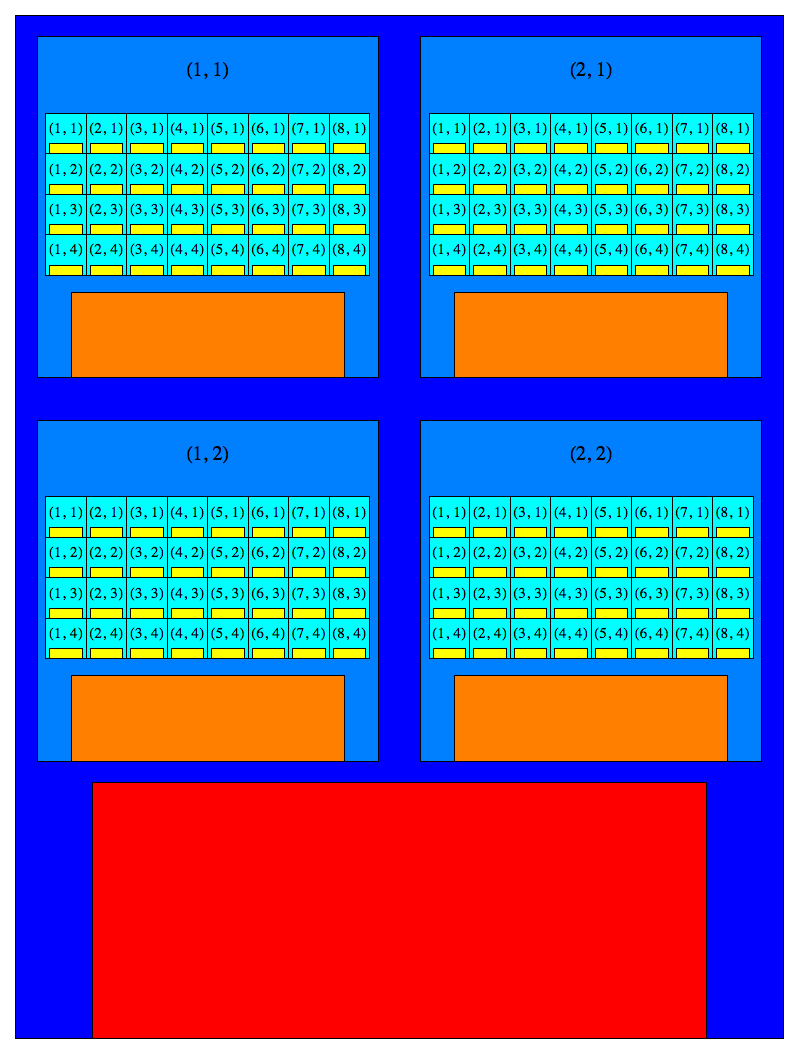
\includegraphics[width=0.83\textwidth]{Figures/gpu_arc.png}
\caption[Architecture of a GPU]
{Architecture of a GPU. Organization of threads and blocks in the grid, and the location of different memory types within them. The grid is coloured dark blue, blocks are coloured light blue, and threads are coloured cyan. The global memory is coloured red, shared memory is coloured orange, and register memory is coloured yellow. The numbers in parenthesis indicate the block or thread's $blockIdx$ or $threadIdx$ variables. In this particular case, $blockDim=(8,4)$ and $gridDim=(2,2)$. A thread is able to access memory that is inside its registers, but not the registers of other threads, and memory that is inside the shared memory of its block, but not the shared memory of other blocks. All threads can access all of the global memory.}
\label{fig:gpuarc}
\end{figure}

\subsection{Occupancy and Performance}
\label{sec:gpuocc}
Having described the various resources, we can talk about how they can be used most effectively. The occupancy of a kernel is the number of warps that are actually able to run on a SM divided by the maximum possible warps an SM can run. Occupancy is important, as it determines the maximum number of blocks, and thus threads that are able to run simultaneously. The occupancy of a kernel is determined by three factors: the block size, the amount of shared memory per block, and the number of registers used per thread. While block size and shared memory are explicitly set by the programmer, it is next to impossible to guess how registers will be used before compile time. Thankfully, there are compiler flags that will display this information.

Armed with the resources our kernel will need, we can now determine its occupancy. The ``CUDA Occupancy Calculator" is an Excel spreadsheet provided by NVIDIA and is an indispensable tool. We can input the needed resources and the hardware generation of our card and then receive the occupancy of the current resource configuration, where the bottleneck of the current configuration is, as well as information on how the occupancy will change upon tweaking the configuration. In some sense, the best block size is determined by how the other resources are used. Therefore, in order to maximize the occupancy, we must first make sure that we are correctly using the memory provided.

Registers are the fastest memory available, but they are also the easiest to overuse. Therefore, they are best suited for small variables that need to be referenced frequently, such as accumulators. Shared memory is best used for storing large sections of non-contiguous data stored in the global memory. Finally, data that is able to be stored such that it can be accessed effectively, or is infrequently used, might best be left in the global memory.

As with everything, these rules are only guidelines. The best resource configuration will be individual not only to every kernel, but also to the GPU it is to be run on. The best way to maximize the efficiency of a calculation is to make minor alterations to where data is stored and play around with the code. Finally, it might not always be the best idea to maximize the occupancy of a kernel. If the bottleneck is not the actual calculation, but how fast the data can be read, then it might be advantageous to fill up the registers and shared memory as much as possible and have a very low occupation.

\subsection{Matrix Multiplication Example}
To complete the introduction to CUDA programming, we will go over a real example of CUDA Fortran code. For our example, we will examine code that performs matrix multiplication on matrices of arbitrary dimensions. This makes use of all the concepts we've covered so far, so it will be a good exercise to examine. The code is given below.
\lstinputlisting[caption={Matrix multiplication kernel}]{code_snippets/mat_mul.cuf}

Lines 1 - 43 define a module which contains a matrix multiplication kernel. The kernel takes the matrices \texttt{inputA} and \texttt{inputB}, multiplies them, and stores the result in \texttt{output}. The kernel has the \texttt{{\color{myblue}{attributes}}(global)} attribute, which means that it can be called from either device or host code. \texttt{rowA}, \texttt{colA}, \texttt{rowB}, and \texttt{colB} are the rows and columns of \texttt{inputA} and \texttt{inputB}. Because they are small and don't change over the course of the calculation, they get stored in a special memory type called constant memory. This is a small cache of read only memory that is 64KB in size and allows for constant values to be read very quickly. There are two shared variables, \texttt{s\_tileA} and \texttt{s\_tileB}. Each of these are square matrices with dimensions of \texttt{block\_dim} and these will be used to store sections or ``tiles" of \texttt{inputA} and \texttt{inputB} respectively. We want each thread to do all the calculations needed to compute a simple element of \texttt{output}. Line 13 and 14 use the \texttt{threadIdx}, \texttt{blockDim}, and \texttt{blockIdx} variables so that each thread gets a unique combination of \texttt{x} and \texttt{y} values. \texttt{x} corresponds to a row of the \texttt{output} matrix and \texttt{y} corresponds to a column, so each thread is then uniquely mapped to an element of \texttt{output}. We will see in the host code how these index values are determined, but for now it is sufficient to know that there will be at least as many threads as elements of \texttt{output}.

Lines 17 - 37 are where the actual calculation takes place. For each iteration of the loop, a different tile of \texttt{inputA} and \texttt{inputB} is fetched from the global memory and stored into the shared memory. The reason for using this tiling approach can be seen when we consider how the threads must read \texttt{inputB}. If we did not use shared memory, the loop would just be \texttt{total {\color{myyellow}{=}} total {\color{myyellow}{+}} inputA(x, i) {\color{myyellow}{*}} inputB(i, y)}. In this case, access to \texttt{inputA} is coalesced, but access to \texttt{inputB} is not. Therefore, the kernel will be stunted due this unoptimized memory usage. Instead, we load tiles in a coalesced manner into the shared memory, synchronize the threads, and then read through the shared memory in an uncoalesced fashion which carries no penalty. At the end of each loop, the tiles are moved in the \texttt{y} direction for \texttt{inputA} and in the \texttt{x} direction for \texttt{inputB}, and the process repeats. Notice how it is possible that a tile might fall on the boundary of an \texttt{input} matrix. This is why there are checks to make sure the coordinates of the tile don't exceed the boundaries of a matrix so we don't start reading garbage.

In the host code on lines 45 - 102, we have two sets of variables, those for the host and those for the device. Notice how device variables have the \texttt{{\color{mygreen}{device}}} attribute. For clarity, they are given the same name as their host variables but with a \texttt{d\_} prefix. We now assign constant variables from line 5 to arbitrary values. Next we set up the random number generator, allocate the host matrices memory, and randomly initialize the input matrices. Then the device variables are allocated memory and the host data is then uploaded to the GPU. The block and grid dimensions are set up on lines 87 and 88. \texttt{blockDim} and \texttt{gridDim} are variables of \texttt{{\color{mygreen}{type}}(dim3)} which is a tuple that is defined in the \texttt{cudafor} module. The block has two dimensions containing \texttt{block\_dim}$^{2}$ threads. The grid also has two dimensions, and as we need one thread per element of \texttt{output} we perform a calculation which returns the minimum number of blocks that will cover it. Finally, we launch the kernel on line 90 using the \texttt{\color{myyellow}{<<< >>>}} operators to provide the grid and block dimensions, download the result from the GPU, and deallocate the memory.

\section{Program flow in cudaDFRATOM}
In this section, the control flow of a typical calculation is given.

\textit{Step 1}. The input file is read by the \textit{\textbf{intin}} subroutine. If needed, the basis set and open-shell configurations are calculated by \textit{\textbf{formbs}} and \textit{\textbf{find\_bin\_configurations}} respectively. The options set in the input file are rewritten to stdout.

\textit{Step 2}. The calculation of small arrays and other constants is performed by \textit{\textbf{calc\_parameters}} and \textit{\textbf{bsnorm}}. \textit{\textbf{calc\_parameters}} calls \textit{\textbf{bcoef}} and \textit{\textbf{setvc}}.

\textit{Step 3}. The mapping of threads to the unrolled one and two-electron integral matrixes are calculated by \textit{\textbf{lmpqrsa}} on the GPU. All other data from step 1 and 2 is then uploaded to the GPU.

\textit{Step 4}. The one and two electron integrals are calculated on the GPU by \textit{\textbf{eint1gpu}} and \textit{\textbf{eint2gpu}} respectively.

\textit{Step 5}. The initial guess of the density matrix is calculated by \textit{\textbf{guess}} on the GPU. This is done by the diagonalization of the one-electron Hamiltonian matrix.

\textit{Step 6}. \textit{\textbf{scfiter}} then performs the SCF iterations until convergence of the density matrix has been reached, or the maximum number of iterations has been reached. SCF is performed with cuSOLVER functions, as well as a few custom helper functions. The converged eigenvectors, values, and energies are downloaded from the GPU and then written to stdout.

\textit{Step 7} (optional). If jobtyp=`bsopt', then an optional basis set optimization is carried out. This starts by assigning pointers to variables on the CPU and GPU through \textit{\textbf{hookup\_cpu}} and \textit{\textbf{hookup\_gpu}}. Then, the four well-tempered basis set (WTBS) parameters are optimized by \textit{\textbf{newuoa}}. \textit{\textbf{newuoa}} calls \textit{\textbf{calc\_energy}} which essentially reconstructs the basis set from new parameters from \textit{\textbf{newuoa}}, then repeats steps 2 - 6 and feeds the energy back into \textit{\textbf{newuoa}}. This repeats until optimal WTBS parameters have been found.

\section{Alterations of DFRATOM for CUDA}
While almost all of the code from the original DFRATOM\cite{MATSUOKA2001218} was modified in some way, the most extreme changes were the integral evaluation and the formation of the P and Q matrixes. Therefore, we will discuss these changes in detail in this section.

\subsection{Two-electron Integrals}
The original DFRATOM calculates the two electron integrals with a long series of nested \textbf{for} loops. Working from the outside in, the indices of the loops are $L$, $P$, $Q$, $M$, $R$, and $S$ where $L$ and $M$ are spinor symmetries, $P$ and $Q$ are basis functions of symmetry $L$, and $R$ and $S$ are basis functions of symmetry $M$. The pseudocode for these is shown in Algorithm \ref{origcode} where $nsym$ is the total number of symmetries, and $nbs(i)$ is the number of basis functions for symmetry species $i$. Thus, each set of J and K integrals is uniquely defined by its $L$, $M$, $P$, $Q$, $R$, and $S$ values. In order to have an effective CUDA implementation of this algorithm, we need to find a way to map these six numbers to CUDA threads. The simplest approach would be to map the values of $L$, $P$, and $Q$ onto the $threadIdx.x$, $threadIdx.y$, and $threadIdx.z$ variables for each thread, launch the needed number of blocks, and then have each thread loop over the remaining indices. The pseudocode for this can be seen in Algorithm \ref{easycode}. A similar method is employed by many other programs, and for larger systems it works perfectly well. But because this program is for only single atoms, problems begin to appear.

\begin{algorithm}
\caption{The original }
\label{origcode}
\begin{algorithmic}
\FOR{$L = 1$ to $nsym$}
	\FOR{$P = 1$ to $nbs(L)$}
		\FOR{$Q = 1$ to $P$}
			\FOR{$M = 1$ to $L$}
				\IF{$L = M$}
					\STATE{$maxr$ = $P$}
				\ELSE
					\STATE{$maxr$ = $nbs(M)$}
				\ENDIF
				\FOR{$R = 1$ to $maxr$}
					\IF{$(L = M)$ \AND $(P = R)$}
						\STATE{$maxs$ = $Q$}
					\ELSE
						\STATE{$maxs$ = $R$}
					\ENDIF
					\FOR{$S = 1$ to $maxs$}
						\STATE{compute the J and K integrals of $L$, $M$, $P$, $Q$, $R$, and $S$}
					\ENDFOR
				\ENDFOR
			\ENDFOR
		\ENDFOR
	\ENDFOR
\ENDFOR
\end{algorithmic}
\end{algorithm}

\begin{algorithm}
\caption{Easy code}
\label{easycode}
\begin{algorithmic}

\STATE{$L = threadIdx.x + (blockIdx.x - 1) * blockDim.x$}
\STATE{$P = threadIdx.y + (blockIdx.y - 1) * blockDim.y$}
\STATE{$Q = threadIdx.z + (blockIdx.z - 1) * blockDim.z$}
\STATE{}
\IF{$(L \leq nsym)$ \AND $(P \leq nbs(L))$ \AND $(Q \leq P)$}
			\FOR{$M = 1$ to $L$}
				\IF{$L = M$}
					\STATE{$maxr$ = $P$}
				\ELSE
					\STATE{$maxr$ = $nbs(M)$}
				\ENDIF
				\FOR{$R = 1$ to $maxr$}
					\IF{$(L = M)$ \AND $(P = R)$}
						\STATE{$maxs$ = $Q$}
					\ELSE
						\STATE{$maxs$ = $R$}
					\ENDIF
					\FOR{$S = 1$ to $maxs$}
						\STATE{compute the J and K integrals of $L$, $M$, $P$, $Q$, $R$, and $S$}
					\ENDFOR
				\ENDFOR
			\ENDFOR
\ENDIF
\end{algorithmic}
\end{algorithm}

The first problem arises due to warp divergence: as the maximum values of $M$, $R$, and $S$ depend on $L$, $P$, and $Q$, different threads will have a different number of loops to complete than others. Because a streaming multiprocessor (SM) must finish the block it is currently working on before it can grab another, there is the possibility that most of the threads in a block are idling while waiting for others in the same block to finish. The second problem with this method is that there will always be several blocks which have threads that remain idle throughout the block's runtime, no matter what. This can be seen more clearly in Figure \ref{fig:naivelayout}. The third problem with this is that with the maximum values for $L$, $P$, and $Q$ available for a single atom, there might not even be enough combinations to completely fill the GPU. While all of these issues begin to disappear once the number of integrals to evaluate becomes large enough, we are still very much in the range where they are in play. Therefore a smarter algorithm had to be used.

\begin{figure}[h!]
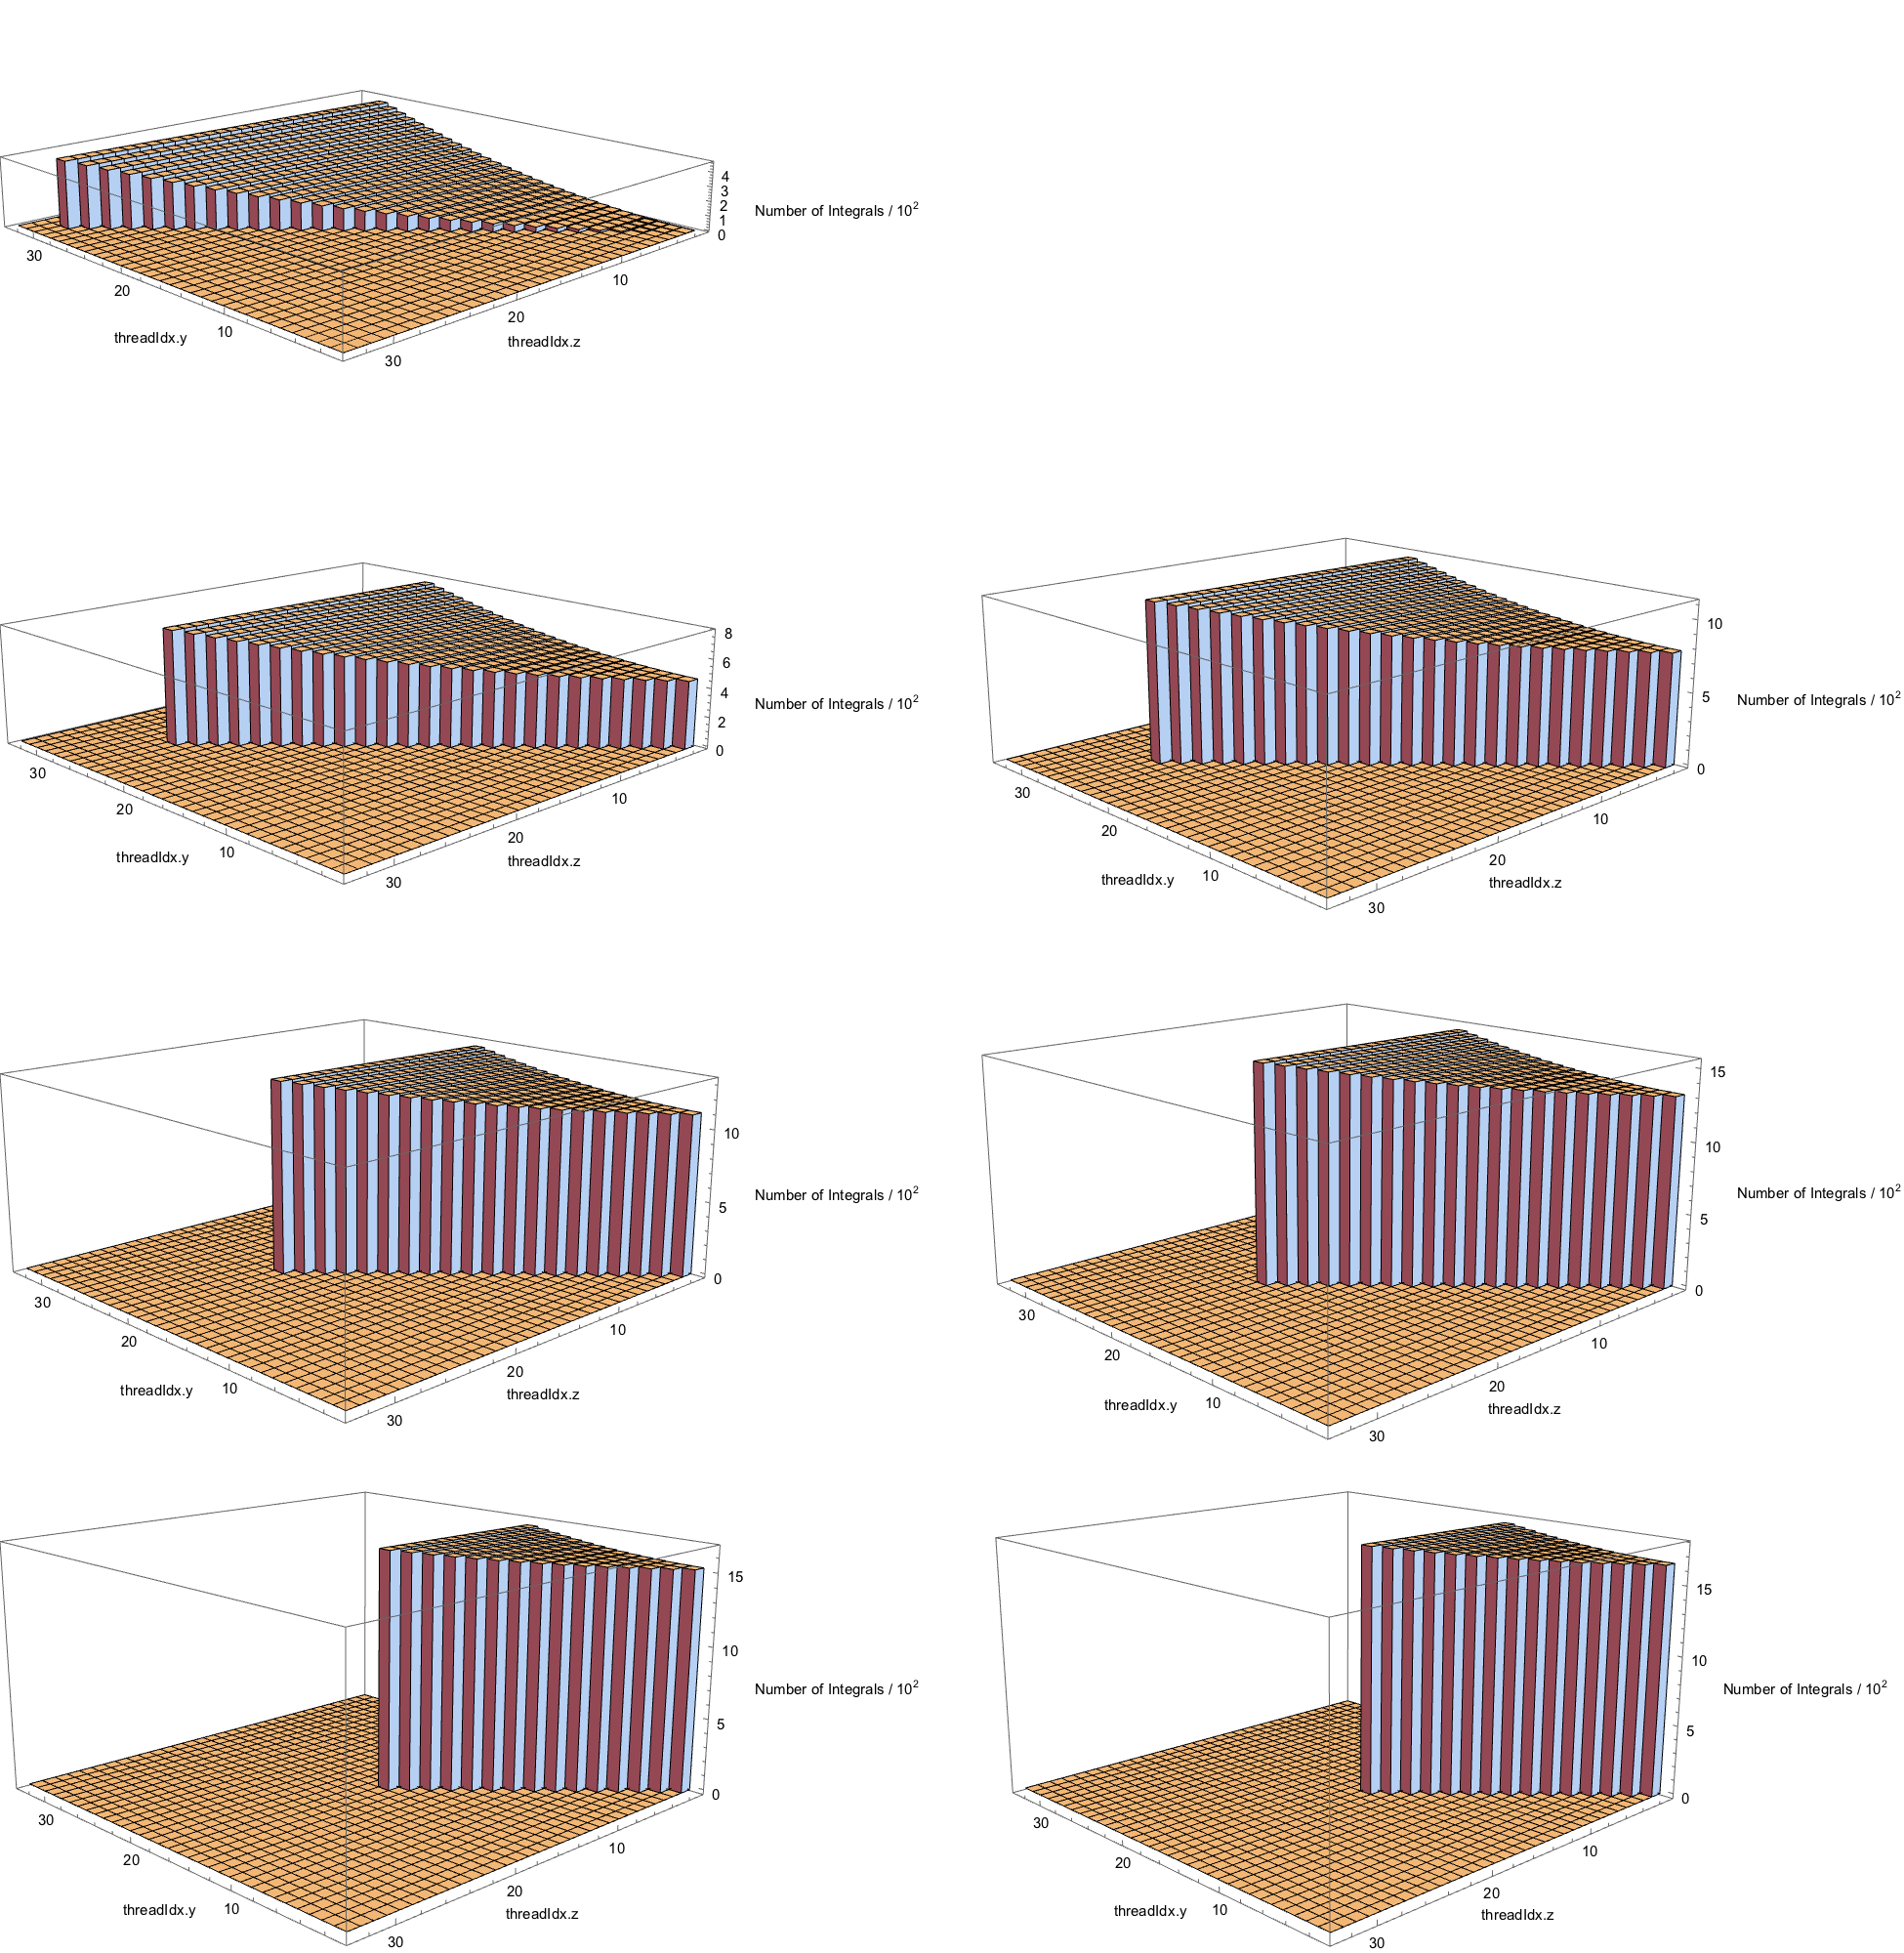
\includegraphics[width=1\textwidth]{Figures/30_25_20_15_naive_layout.png}
\caption[Two-electron integral layout: naive implementation.]
{Two-electron integral layout: naive implementation. Mapping of integrals to threads using Algorithm \ref{easycode}. The basis set used had $nsym = 7$ with $nbs(i)=(30,25,25,20,20,15,15)$. The $blockDim = (1, 32, 32)$ and $gridDim = (7, 1, 1)$. Each histogram is one block of threads, where the horizontal axes are the $threadIdx.y$ and $threadIdx.z$ variables, and the vertical axis is the number of Two-Electron Integrals it must compute. Notice that in all blocks there are threads that calculate no integrals and therefore are idle throughout the lifetime of the block. Also note that the number of integrals each thread must calculate grows both from block to block, and from thread to thread within a block. Both of these factors make this algorithm an undesirable choice.}
\label{fig:naivelayout}
\end{figure}

The second problem can be solved by restricting the dimensionality of the solution instead of the using the three dimensional one of Algorithm \ref{easycode}. We might consider using a two dimensional solution, but then we still will have blocks with idle threads which can be seen in Figure \ref{fig:genmatblock}. By restricting ourselves to only using $threadIdx.x$, we ensure that only the last block to run will have the possibility of having threads remaining idle throughout the block's runtime as shown in Figure \ref{fig:genvecblock}. 

The first and third problems can be solved by having each thread calculate one and only one set of J and K integrals. If we start with a valid combination of $L$, $M$, $P$, $Q$, $R$, and $S$ values, we can very easily figure out which thread will calculate that set of integrals by using the following equations:

\begin{figure}[h!]
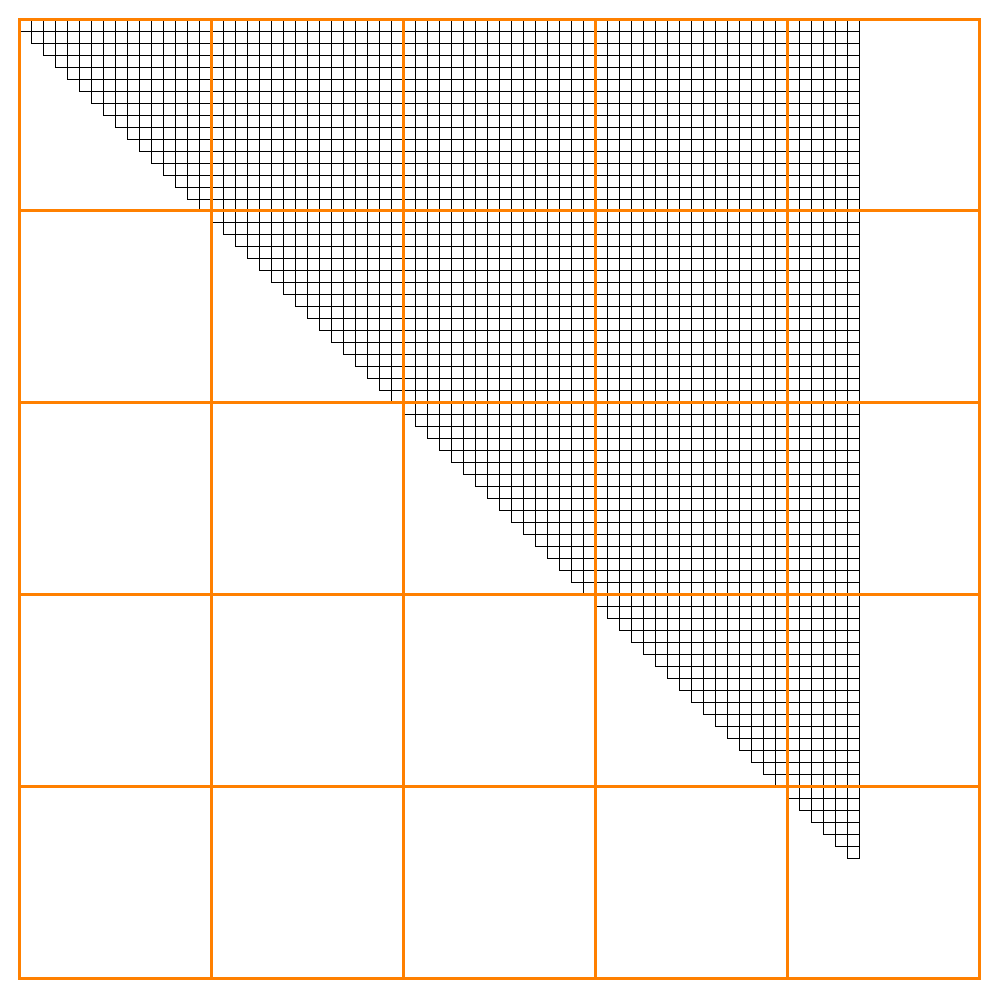
\includegraphics[width=1\textwidth]{Figures/gen_mat_block_layout.png}
\caption[Two-electron integral layout: 2D blocks and grid]
{Two-electron integral layout: 2D blocks and grid. Orange lines indicate the border of blocks. Notice that many blocks have idle threads.}
\label{fig:genmatblock}
\end{figure}

\begin{figure}[h!]
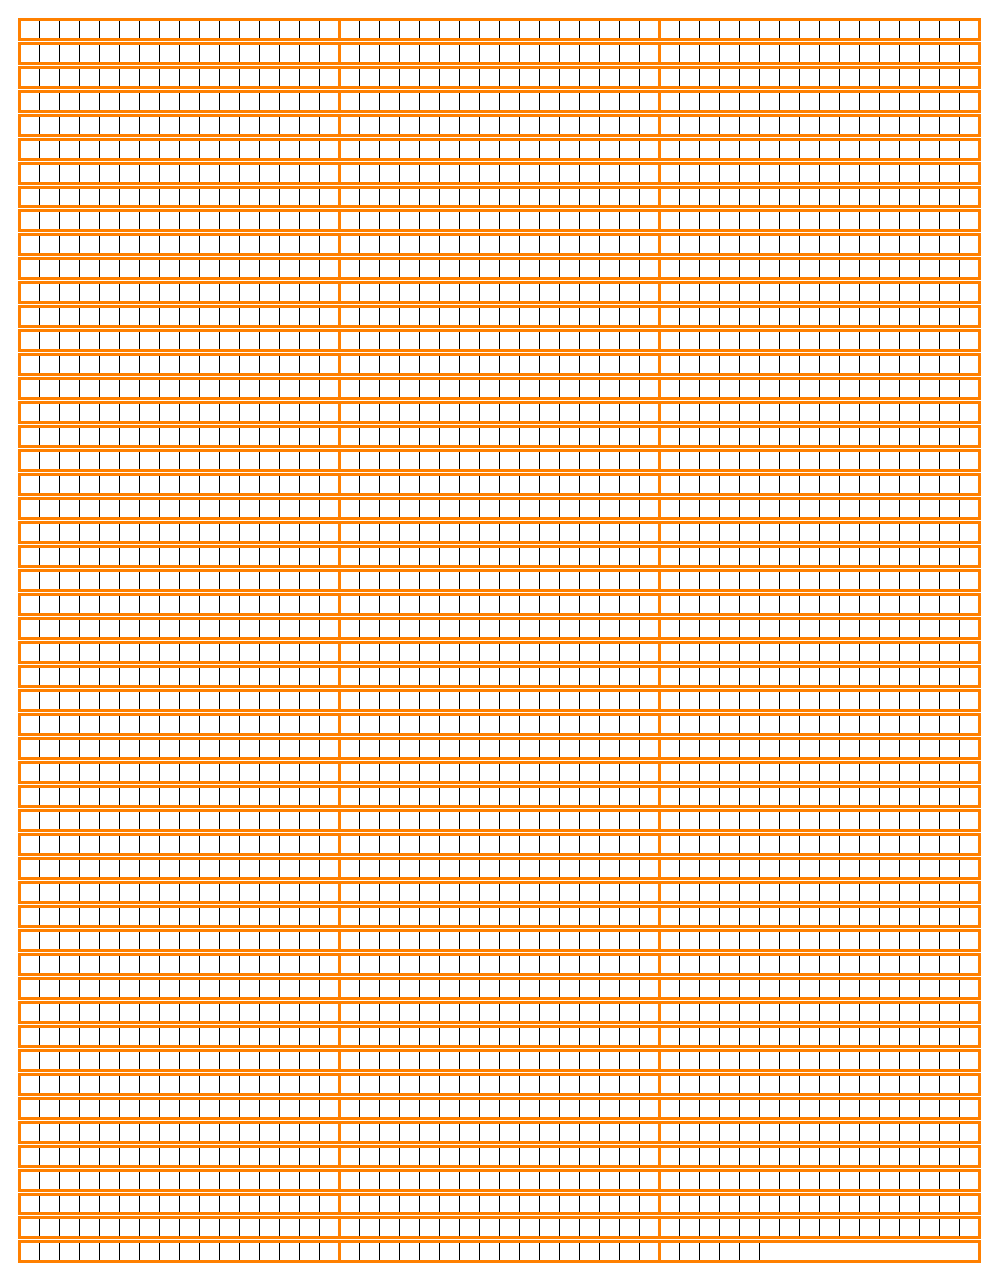
\includegraphics[width=1\textwidth]{Figures/gen_vec_block_layout.png}
\caption[Two-electron integral layout: 1D blocks and grid]
{Two-electron integral layout: 1D blocks and grid. Orange lines indicate the border of blocks. Notice that only the last block contains idle threads.}
\label{fig:genvecblock}
\end{figure}

\begin{equation}
\label{nprime}
n'(j) = \frac{j^{2}+j}{2}
\end{equation}

\begin{equation}
\label{ylpq}
y = n'(nbs(L - 1)) + n'(P - 1) + Q
\end{equation}

\begin{equation}
\label{xmrs}
x = n'(nbs(M - 1)) + n'(R - 1) + S
\end{equation}

\begin{equation}
\label{numtothread}
i = n'(x) + y
\end{equation}

\begin{equation}
\label{imax}
i_{max} = n'(\sum^{nsym}_{j = 1}n'(nbs(j)))
\end{equation}

where $nbs(0) = 0$ and $i=threadIdx.x + (blockIdx.x - 1) * blockDim.x$. Starting with a value of $i$ and working our way back is a much more challenging task. It becomes easier if we reframe it in the following way.

\clearpage

Consider Figures \ref{fig:eint2mat} and \ref{fig:eint2vec}. Figure \ref{fig:eint2mat} shows the top half of the symmetric two-electron integral matrix for a problem with $nsym = 2$ and 3 basis function for symmetry one, and 2 for symmetry two. Figure \ref{fig:eint2vec} shows the same but mapped onto a vector representation. In each element of both figures there is a set of seven numbers. The top two are $L$ and $M$, then $P$ and $Q$, then $R$ and $S$, and the last number is the value of $i$ for the thread calculating that integral. With this, it can be seen from the matrix representation that each element in the same row have the same $M$, $R$, and $S$ values and the elements in the same column have the same $L$, $P$, and $Q$ values. Therefore, finding out which column the element belongs to gives us the value for $y$, and finding the row give us the value of $x$. This can be done with the binary search algorithm shown in Algorithm \ref{bsxy}.

\begin{figure}[h!]
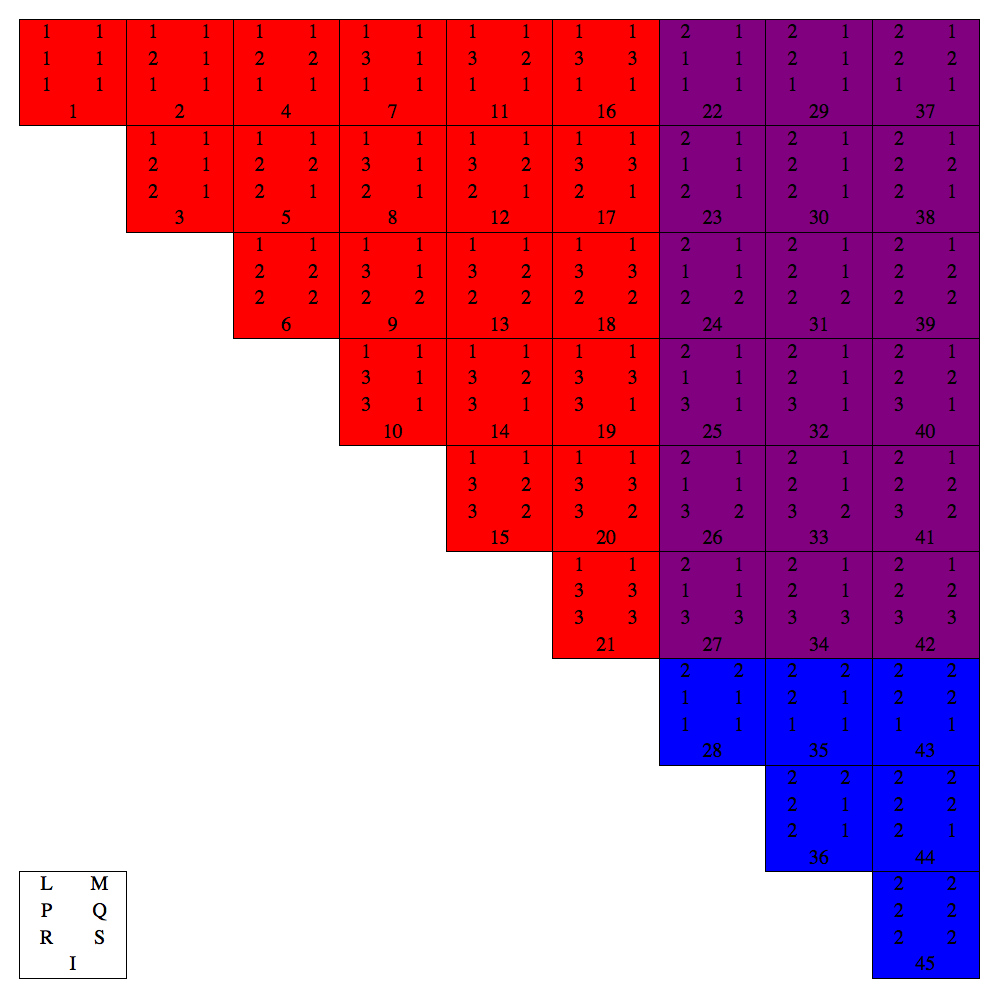
\includegraphics[width=1\textwidth]{Figures/eint2_mat.png}
\caption[Two-electron integral matrix as a matrix]
{Two-electron integral matrix as a matrix: The top triangle of the two-electron symmetric matrix in a matrix representation. In this instance, the total number of symmetries is 2, with 3 basis functions for the first symmetry and 2 basis functions for the second. The key for translating the numbers in each box into the $L$, $M$, $P$, $Q$, $R$, and $S$ values is given in the bottom left. Notice how all rows have the same $M$, $R$, and $S$ values, while all columns have the same $L$, $P$, and $Q$ values. For clarity, the boxes have been coloured, based on the spinor symmetries that they contain.}
\label{fig:eint2mat}
\end{figure}

\begin{figure}[h!]
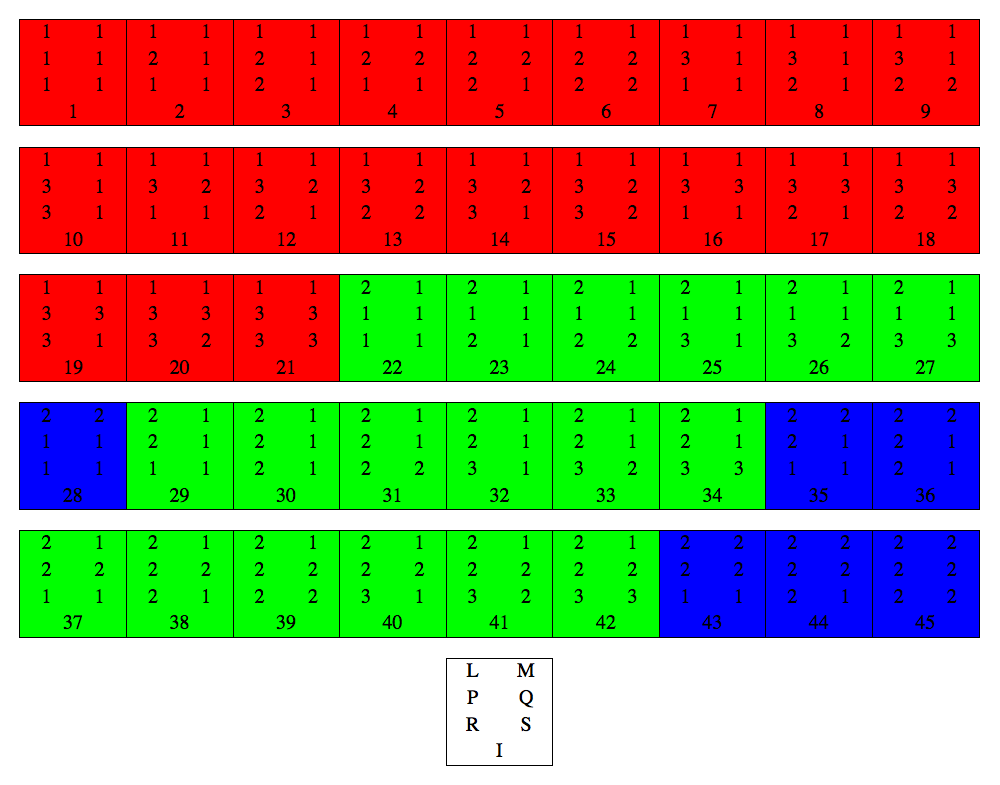
\includegraphics[width=1\textwidth]{Figures/eint2_vec.png}
\caption[Two-electron integral matrix as a vector]
{Two-electron integral matrix as a vector: The top triangle of the two-electron symmetric matrix in a vector representation. In this instance, the total number of symmetries is 2, with 3 basis functions for the first symmetry and 2 basis functions for the second. The key for translating the numbers in each box into the $L$, $M$, $P$, $Q$, $R$, and $S$ values is given in the bottom center. Notice how the $L$, $M$, $P$, $Q$, $R$, and $S$ values are much harder to predict than from the matrix representation. For clarity, the boxes have been coloured based on the spinor symmetries that they contain. Gaps between rows are used to reinforce that the elements are not connected like a matrix.}
\label{fig:eint2vec}
\end{figure}


\begin{algorithm}[h!]
\caption{Binary search for $x$ and $y$}
\label{bsxy}
\begin{algorithmic}

\IF{$theadIdx.x \leq nsym$}
	\STATE{$s\_nsym = nsym$}
	\STATE{$s\_nbs(threadIdx.x) = nbs(threadIdx.x)$}
	\STATE{$s\_nprime(threadIdx.x) = n'(s\_nbs(threadIdx.x))$}
\ENDIF

\STATE{call \textbf{syncthreads}}

\STATE{$i =  threadIdx.x + (blockIdx.x - 1) * blockDim.x$}
\IF{$i \leq i_{max}$}
	\STATE{$low = 1$}
	\STATE{$high = \textbf{sum}(s\_nprime(1:s\_nsym))$}
	\WHILE{$low \leq high$}
		\STATE{$mid = \frac{(low + high)}{2}$}
		\STATE{$lownum = \frac{(mid - 1)(mid - 2)}{2} + mid$}
		\STATE{$highnum = lownum - 1 + mid$}
		\IF{$(i \leq highnum)$ \AND $(i \geq lownum)$}
			\STATE{$y = mid$}
			\STATE{\textbf{exit}}
		\ELSIF{$i > highnum$}
			\STATE{l$ow = mid + 1$}
		\ELSIF{$i < lownum$}
			\STATE{$high = mid - 1$}
		\ENDIF
	\ENDWHILE
	\STATE{$x = i - lownum + 1$}
\ENDIF

\end{algorithmic}
\end{algorithm}

In this algorithm, variables with the $s\_$ prefix refer to those in the shared memory, and $lownum$ and $highnum$ refer to the minimum and values that $i$ could have for the current guess ($mid$) of $y$. From here, $L$ can be found with Algorithm \ref{bsL}, and $P$ and $Q$ can be found with Algorithm \ref{bsPQ}. The same set of algorithms can then be used to get $M$, $R$, and $S$ by substituting the relevant variables. If there is sufficient global memory available, these values can be stored and referred to later as needed. Otherwise, they could be calculated on the fly as needed. Because binary search scales as $\mathcal{O}(n\log{}n)$, this should ensure that this remains a fast method of mapping threads to integrals for large problems as well. With some alterations, this method could also apply to molecular symmetries and not only to a single atom. For instance in the C$_{1}$ symmetry, all possible combinations of four basis functions must be used (ignoring those that appear on the bottom triangle of the two electron integral matrix of course). We could simply remove the search for $L$ and $M$, have the initial value of $high$ in Algorithm \ref{bsPQ} be the total number of basis functions, and remove the \textbf{sum}$(s\_nprime(1:L-1)$ term from $lownum$.

\begin{algorithm}
\caption{Binary search for $L$}
\label{bsL}
\begin{algorithmic}

\STATE{$i =  threadIdx.x + (blockIdx.x - 1) * blockDim.x$}
\IF{$i \leq i_{max}$}
	\STATE{$low = 1$}
	\STATE{$high = s\_nsym$}
	\WHILE{$low \leq high$}
		\STATE{$mid = \frac{(low + high)}{2}$}
		\STATE{$lownum = 1 + \textbf{sum}(s\_nprime(1:mid-1)$}
		\STATE{$highnum = lownum - 1 + s\_nprime(mid)$}
		\IF{$(i \leq highnum)$ \AND $(i \geq lownum)$}
			\STATE{$L = mid$}
			\STATE{\textbf{exit}}
		\ELSIF{$y > highnum$}
			\STATE{$low = mid + 1$}
		\ELSIF{$y < lownum$}
			\STATE{$high = mid - 1$}
		\ENDIF
	\ENDWHILE
\ENDIF

\end{algorithmic}
\end{algorithm}

\begin{algorithm}
\caption{Binary search for $P$ and $Q$}
\label{bsPQ}
\begin{algorithmic}

\STATE{$i =  threadIdx.x + (blockIdx.x - 1) * blockDim.x$}
\IF{$i \leq i_{max}$}
	\STATE{$low = 1$}
	\STATE{$high = s\_nbs(L)$}
	\WHILE{$low \leq high$}
		\STATE{$mid = \frac{(low + high)}{2}$}
		\STATE{$lownum =  \frac{(mid - 1)(mid - 2)}{2} + mid + \textbf{sum}(s\_nprime(1:L-1))$}
		\STATE{$highnum = lownum + mid - 1$}
		\IF{$(i \leq highnum)$ \AND $(i \geq lownum)$}
			\STATE{$P = mid$}
			\STATE{\textbf{exit}}
		\ELSIF{$y > highnum$}
			\STATE{$low = mid + 1$}
		\ELSIF{$y < lownum$}
			\STATE{$high = mid - 1$}
		\ENDIF
	\ENDWHILE
	\STATE{$Q = y - lownum + 1$}
\ENDIF

\end{algorithmic}
\end{algorithm}

From here, the new code for evaluating the integrals remains largely the same as the original, except for some minor changes to allow for more efficient global or shared memory access. We also use a process referred to as ``grid-stride looping" where all these binary search algorithms have their \textbf{if} $i \le i_{max}$ \textbf{then} removed, and then are placed within the following loop: \textbf{for} $i = threadIdx.x + (blockIdx.x - 1) * blockDim.x$ to $i_{max}$, $i \mathrel{+}= blockDim.x * gridDim.x$ \textbf{do}. If we know the occupancy of the algorithm on the GPU beforehand, we can launch exactly the number of blocks that will fill the GPU. This reduces the overhead of block swapping and lets us further eke out some performance.

\subsection{Density Matrix Formation}
The term in parenthesis in Equation \ref{FOCKM} corresponds to the non-relativistic density matrix. But as we are interested in relativistic calculations, it will need to be altered. Firstly, because a relativistic wavefunction has both large and small components, so too does its density matrix. Therefore, it will have two dimensions that span from 1 to $2K$ where dimensions 1 to $K$ are the large components and the rest are for small components. Secondly, the factor of 2 is replaced by the number of electrons that can occupy spinors of symmetry $\mu$. The density matrix's matrix and vector representations are shown in Figures \ref{fig:dtmxmat} and \ref{fig:dtmxvec} respectively. The mathematical form of the density matrix is given in Equation \ref{RDCMX}\cite{MATSUOKA2001218}

\begin{equation}
\label{RDCMX}
\textbf{D$_{\textbf{C}r,s}$} =N_{\mu}\sum^{occ}_{a=1}\textbf{C}_{r,a}\textbf{C}^{*}_{s,a}
\end{equation}

\begin{figure}
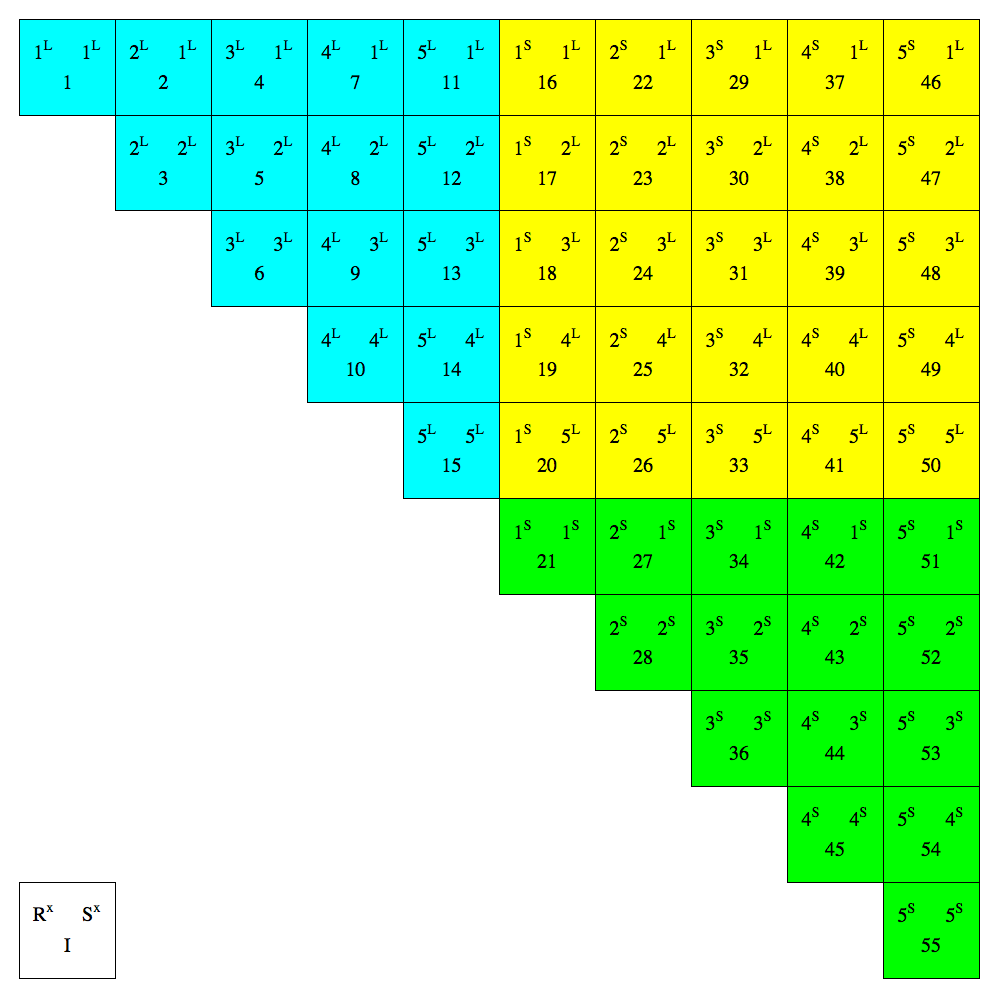
\includegraphics[width=1\textwidth]{Figures/dtmx_mat.png}
\caption[Density matrix as a matrix]
{Density matrix as a matrix. The top triangle of the symmetric density matrix in a matrix representation. The key for translating the numbers in each box into the $R$ and $S$ values is given in the bottom right. All active symmetries would have a similar, separate matrix. For clarity, the elements have been colorized based on the combination of large and small components they contain.}
\label{fig:dtmxmat}
\end{figure}

\begin{figure}
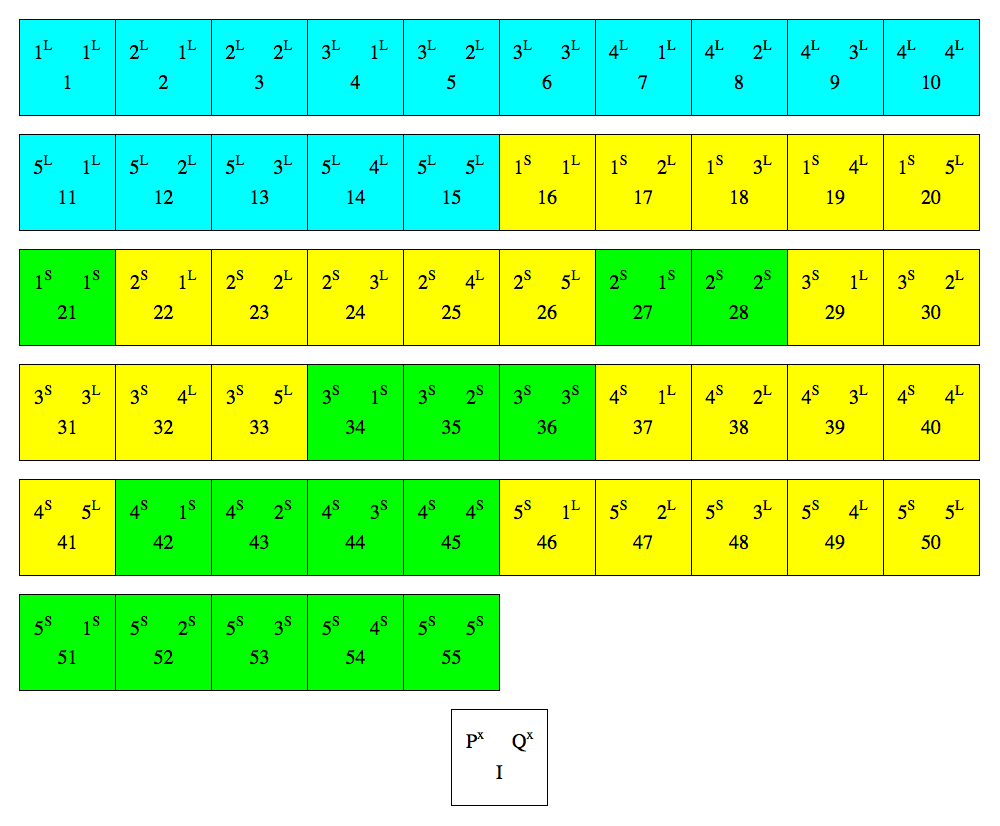
\includegraphics[width=1\textwidth]{Figures/dtmx_vec.png}
\caption[Density matrix as a vector]
{Density matrix as a vector. The top triangle of the symmetric density matrix in a vector representation. The key for translating the numbers in each box into the $R$ and $S$ values is given in the bottom left. All active symmetries would have a similar, separate vector that continue one after the other. For clarity, the elements have been colorized based on the combination of large and small components they contain.}
\label{fig:dtmxvec}
\end{figure}


where $N_{i}$ is the number of electrons that occupy a closed shell of symmetry $i$. \textbf{D$_\textbf{O}$} is similar to this and is shown below.

\begin{equation}
\label{RDOMX}
\textbf{D$_{\textbf{O}r,s}$} =N_{i}\textbf{C}_{r,(occ+1)}\textbf{C}^{*}_{s,(occ+1)}
\end{equation}

where $N_{i}$ is equal to the number of electrons in the open shell. Note that in this program, only the most energetic shell of any symmetry can be open.

The total density matrix is $\textbf{D$_{\textbf{T}}$} =  \textbf{D$_{\textbf{C}}$} + \textbf{D$_{\textbf{O}}$}$

\subsubsection{P and Q Supermatrices}
\label{sec:PQmeth}
With the density matrices in hand we can begin to combine the two-electron integrals from the previous section. These integrals have the following form.\cite{MATSUOKA2001218}

\begin{equation}
\label{2EINTS}
\begin{split}
\textbf{X}^{1}_{I(pqrs)}	&	= \left(p_{L}q_{L}|r_{L}s_{L}\right) - \frac{1}{2}\left[\left(p_{L}r_{L}|q_{L}s_{L}\right) + \left(p_{L}s_{L}|q_{L}r_{L}\right)\right]	\\
\textbf{X}^{2}_{I(pqrs)}	&	= \left(p_{L}q_{L}|r_{S}s_{S}\right)																	\\
\textbf{X}^{3}_{I(pqrs)}	&	= \left(p_{S}q_{S}|r_{L}s_{L}\right)																	\\
\textbf{X}^{4}_{I(pqrs)}	&	= -\left(p_{L}r_{S}|q_{S}s_{L}\right)																	\\
\textbf{X}^{5}_{I(pqrs)}	&	= -\left(p_{L}s_{S}|q_{S}r_{L}\right)																	\\
\textbf{X}^{6}_{I(pqrs)}	&	= -\left(p_{S}r_{L}|q_{L}s_{S}\right)																	\\
\textbf{X}^{7}_{I(pqrs)}	&	= -\left(p_{S}s_{L}|q_{L}r_{S}\right)																	\\
\textbf{X}^{8}_{I(pqrs)}	&	= \left(p_{S}q_{S}|r_{S}s_{S}\right) - \frac{1}{2}\left[\left(p_{S}r_{S}|q_{S}s_{S}\right) + \left(p_{S}s_{S}|q_{S}r_{S}\right)\right]	\\
\end{split}
\end{equation}

where the subscripts $L$ and $S$ refer to the large and small components respectively. $I$ is a function that returns the values of $x$ and $y$ from Equations \ref{ylpq} and \ref{xmrs} where $L=\lambda$ and $M=\mu$. From here, all subscripts of \textbf{X} will be implied to go through this $I$ function.

The \textbf{P} and \textbf{Q} super matrices have a similar layout to the density matrices. The elements of \textbf{P} have the following form\cite{MATSUOKA2001218}

\begin{equation}
\label{PSMTX}
\begin{split}
\textbf{P}^{LL}_{pq}	&	= \sum_{\mu = 1}^{nsym}\sum_{r=1}\sum_{s=1}\left(\textbf{D$^{LL}_{\textbf{T}rs}$}\textbf{X}^{1}_{pqrs} + \textbf{D$^{SS}_{\textbf{T}rs}$}\textbf{X}^{J(pqrs)}_{pqrs}\right)	\\
\textbf{P}^{SS}_{pq}	&	= \sum_{\mu = 1}^{nsym}\sum_{r=1}\sum_{s=1}\left(\textbf{D$^{SS}_{\textbf{T}rs}$}\textbf{X}^{8}_{pqrs} + \textbf{D$^{LL}_{\textbf{T}rs}$}\textbf{X}^{J(pqrs)}_{pqrs}\right)	\\
\textbf{P}^{LS}_{pq}	&	= \sum_{\mu = 1}^{nsym}\sum_{r=1}\sum_{s=1}\left(\textbf{D$^{LS}_{\textbf{T}rs}$}\textbf{X}^{5}_{pqrs} + \textbf{D$^{SL}_{\textbf{T}rs}$}\textbf{X}^{J(pqrs)}_{pqrs}\right)	\\
\textbf{P}^{SL}_{pq}	&	= \sum_{\mu = 1}^{nsym}\sum_{r=1}\sum_{s=1}\left(\textbf{D$^{SL}_{\textbf{T}rs}$}\textbf{X}^{7}_{pqrs} + \textbf{D$^{LS}_{\textbf{T}rs}$}\textbf{X}^{J(pqrs)}_{pqrs}\right)	\\
\end{split}
\end{equation}

where $J(pqrs)$ is an integer function that selects specific definitions of the two-electron integrals from Equation \ref{2EINTS}. How exactly this works is shown in the following sections.

The form of the \textbf{Q} super matrix is almost the same a \textbf{P}, but there will be and additional multiplication of the vector coupling coefficient between the open shells for each summation.

\subsubsection{FORMPQ Algorithm}
Forming the P and Q matrices proved to be the most difficult part of this program to parallelize. Its difficulty was due to the second term in the summations where each \textbf{X} matrix used depends on how far the summation has progressed. Further, each element of \textbf{P} will have the \textbf{X} matrix change at different times. These two factors result in many \textbf{if} statements which GPUs have difficulty handling in parallel. There is also the issue where each element in the $LL$ and $SS$ sections need to loop over every element of the same sections of the density matrix, as do the $LS$ and $SL$ sections. This means that there will be lots of global memory reads unless handled properly. All together, this makes for a very ugly algorithm to parallelize.

Two different attempts were made to try and accelerate this algorithm. Each tried to exploit a different property of GPUs. One attempted to combat the amount of floating point operations to perform by distributing the amount of work to as many threads as possible. This will be referred to as the Multiple Threads Single Element (MTSE) algorithm. The second one tried to deal with the amount of global memory reads by making the most of each read. This will be referred to as Single Thread Single Element (STSE) algorithm. Each will be described in the sections below.

\subsubsection{MTSE Algorithm}
As previously stated, the purpose of the MTSE algorithm is to distribute the amount of work needed to be done to as many threads as possible. This was achieved by having multiple threads each computing two of the multiplications needed for a single element of two matrices in Equation \ref{PSMTX}, and then combining the products of these multiplications in parallel. These two tasks were performed by two separate kernels. Pseudocode showing how each calculates the \textbf{P} matrix is shown in Algorithms \ref{MTSE_K1} and \ref{MTSE_K2} respectively. 

\begin{algorithm}
\caption{Kernel 1 for MTSE}
\label{MTSE_K1}
\begin{algorithmic}

\STATE{$i =  threadIdx.x + (blockIdx.x - 1) * blockDim.x$}
\STATE{$j =  blockIdx.y$}
\STATE{$inttype = blockIdx.z - 1$}
\IF{$i \leq total$}
	\STATE{$l = lpq\_array(i, 1)$}
	\STATE{$p = lpq\_array(i, 2)$}
	\STATE{$q = lpq\_array(i, 3)$}
	\STATE{$fctr = 1.0$}
	\IF{$(p \neq q)$ \AND $(inttype == 0)$}
		\STATE{$fctr = 2.0$}
	\ELSIF{$(p == q)$ \AND $(inttype == 1)$}
		\STATE{$fctr = 0.5$}
	\ENDIF
	\STATE{$loc = \textbf{max}(i, j) + ((\textbf{max}(i, j) - 1) * (\textbf{max}(i, j) - 2) / 2) + \textbf{min}(i, j) - 1$}
	\IF{$(inttype == 0)$}
		\IF{$i>j$}
			\STATE{$k1 = 3$}
			\STATE{$k2 = 2$}
		\ELSE
			\STATE{$k1 = 2$}
			\STATE{$k2 = 3$}
		\ENDIF
		\STATE{$pos1 = locmx(l) + ((p - 1)^2 + p - 1) / 2 + q$}
		\STATE{$pos2 = locmx(l) + ((p - 1 + nbs(l))^2 + p + nbs(l) - 1) / 2 + q + nbs(l)$}
		\STATE{$pLL(i, j) = d(pos1) * fctr * x(1, loc) + d(pos2) * fctr * x(k1, loc)$}
		\STATE{$pSS(i, j) = d(pos1) * fctr * x(k2, loc) + d(pos2) * fctr * x(k8, loc)$}
	\ELSE
		\IF{$i>j$}
			\STATE{$k1 = 4$}
			\STATE{$k2 = 6$}
		\ELSE
			\STATE{$k1 = 6$}
			\STATE{$k2 = 4$}
		\ENDIF
		\STATE{$pos1 = locmx(l) + ((p - 1 + nbs(l))^2 + p - 1 + nbs(l)) / 2 + q$}
		\STATE{$pos2 = locmx(l) + ((q - 1 + nbs(l))^2 + q - 1 + nbs(l)) / 2 + p$}
		\STATE{$pSL(i, j) = d(pos1) * fctr * x(7, loc) + d(pos2) * fctr * x(k1, loc)$}
		\STATE{$pLS(i, j) = d(pos1) * fctr * x(k2, loc) + d(pos2) * fctr * x(5, loc)$}
	\ENDIF
\ENDIF
\end{algorithmic}
\end{algorithm}

\begin{algorithm}
\caption{Kernel 2 for MTSE}
\label{MTSE_K2}
\begin{algorithmic}

\STATE{$i =  threadIdx.x + (blockIdx.x - 1) * blockDim.x * 2$}
\STATE{$inttype = blockIdx.z - 1$}

\IF{$inttype == 0$}
	\IF{$i \leq total$}
		\STATE{$s\_tile(threadIdx.x) = pLL(i, blockIdx.y)$}
	\ELSE
		\STATE{$s\_tile(threadIdx.x) = 0.0$}
	\ENDIF
	\IF{$i + blockDim.x \leq total$}
		\STATE{$s\_tile(threadIdx.x + blockDim.x) = pLL(i + blockDim.x, blockIdx.y)$}
	\ELSE
		\STATE{$s\_tile(threadIdx.x + blockDim.x) = 0.0$}
	\ENDIF
\ELSE
\STATE{Perform a similar instruction on the other $pXY$ or $qXY$ matrices depending on $inttype$}
\ENDIF
\FOR{$j = \textbf{log}_{2}(blockDim.x), j \geq 0, j = j-1$}
	\STATE{call \textbf{syncthreads}}
	\IF{$threadIdx.x \leq 2^{j}$}
		\STATE{$s\_tile(threadIdx.x) = s\_tile(threadIdx.x) + s\_tile(threadIdx.x + 2^{j})$}
	\ENDIF
\ENDFOR	 
\IF{$threadIdx.x == 1$}
	\STATE{$l = lpq\_array(blockIdx.y, 1)$}
	\STATE{$p = lpq\_array(blockIdx.y, 2)$}
	\STATE{$q = lpq\_array(blockIdx.y, 3)$}
	
	\IF{$(inttype == 0)$}
		\STATE{$pos = locmx(l) + ((p - 1)^{2} + p - 1) / 2 + q$}
		\STATE{$istat = \textbf{atomicadd}(pmx(pos), s\_tile(threadIdx.x))$}
	\ELSE
		\STATE{Perform a similar instruction on the other $pXY$ or $qXY$ matrices depending on $inttype$}
	\ENDIF	
\ENDIF

\end{algorithmic}
\end{algorithm}

$inttype$ refers to one or more if the \textbf{P} or \textbf{Q} matrices. In Algorithm \ref{MTSE_K1}, $inttype$ can have a value of 0 or 1, where 0 refers to the $LL$ and $SS$ \textbf{P} or \textbf{Q} matrices, and 1 is the $SL$ and $LS$ matrices.  In Algorithm \ref{MTSE_K2}, $inttype$ can have a values ranging from 0 to 7 where 0 to 3 are the \textbf{P} $LL$, $SS$, $SL$, $LS$ matrices, and the rest are the \textbf{Q} matrices in the same order. $d$ is \textbf{D} in its vector representation and $pos$ are the locations of the $p$ and $q$ elements within it. $locmx$ is an array with 7 elements, and each element is equal to the number of unique $LL$, $SS$, $SL$, $LS$ elements of symmetry $l-1$. $fctr$ accounts for when an element is single or double counted in the summation. $x(\chi, :)$ is the vector representation of \textbf{X$^{\chi}$}, $loc$ is the location of needed $pqrs$ element in the vector, $total$ is the length of one of the dimensions of \textbf{X$^{\chi}$}, and $k1$ and $k2$ are the outputs of the $J$ function from Equation \ref{PSMTX}. Finally, $pXY$ variables are matrices dimension $total \times total$ and store the sum of the two multiplications of the $d$ and $x$ vectors, $pmx$ if the vector representation of the \textbf{P} matrices, and $s\_tile$ is a vector in the shared memory for summing up the elements of each row of the $pXY$ matrices. 

The grid will need to have $\frac{total - 1}{blockDim.x} \times \frac{total - 1}{blockDim.y} \times 2$ dimensions for Algorithm \ref{MTSE_K1} and $\frac{total - 1}{blockDim.x} \times \frac{total - 1}{blockDim.y} \times 8$ for Algorithm \ref{MTSE_K2}. Algorithm \ref{MTSE_K1} is fairly straightforward, but Algorithm \ref{MTSE_K2} could use a little more explanation. It is a ``parallel reduction" algorithm. At the start, each thread loads an element of the relevant $pXY$ array into the shared variable $s\_tile$ and also loads the element that is $blockDim.x$ elements ahead of the original element. Then, in a loop starting from $j= \textbf{log}_{2}(blockDim.x)$ and descending to $j = 0$ threads with a $threadIdx.x$ value of less then $2^{j}$ add the value of  $s\_tile(threadIdx.x + 2^{j})$ to $s\_tile(threadIdx.x)$. The key feature is that the amount of elements that need to be added is reduced by half in every loop. Because it is possible that the total number of elements of $pXY$ needed to sum up for the relevant $pmx$ element could be larger than one block can handle, atomic operations are used to force the final addition to occur serially.

\subsubsection{STSE Algorithm}
The STSE algorithm tries a different approach to this problem than the MTSE algorithm. Instead of trying to spread out the amount of work to do as much as possible, it tries to reduce the amount of global memory reads by making each thread do as much work as it can. This results in fewer blocks, but each block needs to run longer. Giving only the calculations for $pmx$ and when $inttype = 0$, Algorithm \ref{STSE_K} shows how this is done.

\begin{algorithm}
\caption{STSE algorithm}
\label{STSE_K}
\begin{algorithmic}

\STATE{$i =  threadIdx.x + (blockIdx.x - 1) * blockDim.x$}
\STATE{$inttype = blockIdx.z - 1$}
\IF{$i \leq total$}
	\STATE{$l = lpq\_array(i, 1)$}
	\STATE{$p = lpq\_array(i, 2)$}
	\STATE{$q = lpq\_array(i, 3)$}
	\STATE{$fctr = 1.0$}
	\STATE{$loop = 0$}
	\FOR{$j = 1, j \leq (total - 1)/blockDim.x + 1, j = j + 1$}
		\STATE{$mink = 1 + (j - 1) * blockDim.x$}
		\STATE{$maxk = \textbf{min}(j * blockDim.x, total)$}
		\IF{$threadIdx.x + (j - 1) * blockDim.x \leq total$}
			\STATE{$m = lpq\_array(threadIdx.x + (j - 1) * blockDim.x, 1)$}
			\STATE{$r = lpq\_array(threadIdx.x + (j - 1) * blockDim.x, 2)$}
			\STATE{$s = lpq\_array(threadIdx.x + (j - 1) * blockDim.x, 3)$}
			\IF{$(r \neq s)$ \AND $(inttype == 0)$}
				\STATE{$fctr = 2.0$}
			\ENDIF
			\STATE{$s\_d(threadIdx.x, 1) = fctr * d(locmx(m) + ((r - 1)^2 + r - 1) / 2 + s - 1)$}
			\STATE{$s\_d(threadIdx.x, 2) = fctr * d(locmx(m) + ((r - 1 + nbs(m))^2 + r + nbs(m) - 1) / 2 + s + nbs(m))$}
		\ENDIF
		\STATE{$fctr = 1.0$}
		\STATE{call \textbf{syncthreads}}
		\FOR{$k = mink, k \leq maxk, k = k + 1$}
			\IF{$(i \geq k)$ \AND $(inttype == 0)$}
				\STATE{$loc = ((i - 1)^{2} + i - 1) / 2 + k$}
				\STATE{$k1 = 3$}
				\STATE{$k2 = 2$}
			\ELSIF{$(i < k)$ \AND $(inttype == 0)$}
				\STATE{$loop = loop + k - 1$}
				\STATE{$loc = (i^{2} + i) / 2 + loop$}
				\STATE{$k1 = 2$}
				\STATE{$k2 = 3$}
			\ENDIF
			\STATE{$pm1 = pm1 + s\_d(1 + k - mink, 1) * x(1, loc) + s\_d(1 + k - mink, 2) * x(k1, loc)$}
			\STATE{$pm2 = pm2 + s\_d(1 + k - mink, 1) * x(k2, loc) + s\_d(1 + k - mink, 2) * x(k8, loc)$}
		\ENDFOR
		\STATE{call \textbf{syncthreads}}
	\ENDFOR
	\STATE{$pmx(locmx(l) + ((p - 1)^2 + p - 1) / 2 + q) = pm1$}
	\STATE{$pmx(locmx(l) + ((p - 1 + nbs(l))^2 + p + nbs(l) - 1) / 2 + q + nbs(l)) = pm2$}
\ENDIF
\end{algorithmic}
\end{algorithm}

All variables are the same as in Algorithms \ref{MTSE_K1} and \ref{MTSE_K2}, but $inttype$ can only be 0 or 1 (the meanings are the same as in Algorithm \ref{MTSE_K1}). As for the new variables, $s\_d$ is a chunk of $d$ that has been loaded into the shared memory. $mink$ and $maxk$ are used to calculated the sections of $x$ that current chunk of $d$ in shared memory applies to and $loop$ is used to adjust the value of $loc$ if the needed two-electron integral is on the bottom triangle of a \textbf{X} matrix. $pm1$ and $pm2$ are accumulator variables that track the sum of an element of $pmx$ as $d$ is looped through.

Algorithm \ref{STSE_K} has two nested loops. The outer one loops over elements of $d$, loading chunks of it into the shared memory as it goes. The inner one loops over elements of $x$ and performs the multiplications of $d$ and $x$ elements, keeping a running tally of the sum of these multiplications. Something that is not shown in the pseudocode is checking if $l$ and $m$ have open shells. If both of them do, then $qm1$ and $qm2$ will be calculated as well. If only one or neither of them do, then this calculation is skipped. Because most of the shells will be closed, this allows for many calculations to be skipped. Once the inner loop has finished, the next section of $d$ is loaded into the shared memory and then the multiplication of $x$ and $s\_d$ continues. This process goes on until all elements of a row of \textbf{X} have been used.

\section{Discussion}
In this section, the results of GPU resource usage and profiling the various algorithms discussed previously will be presented. For profiling, the radon atom was chosen. Radon was selected because it contains many spinor orbitals and should be a good test of the \kernel{formpq} and \kernel{eint2} kernels on large atomic systems. Some of the smaller basis sets used do not contain a sensible number of basis functions considering the number of electrons that Radon contains. This is not an issue though, as at this stage we are only concerned with how long the calculation takes, and not with how accurate its end result is. Therefore, basis sets use the arbitrarily chosen WTBS parameters of $\alpha = 6.87\times10^{-2}$, $\beta = 1.83$,  $\delta = 3.97$, and $\gamma = 0.78$. Additionally, due to the spherical symmetry of an atom exploited by cudaDFRATOM, the growth of a calculation differs depending on how the basis functions are distributed among the spinor symmetries. Therefore, results are reported in terms of the number of two-electron integrals instead of number of basis functions as is typically done.
\subsection{Resource Usage}
In the case of the work in this thesis, the resource bottleneck for my kernels was almost always the number of registers used per thread. 63 32-bit registers provide only 252 bytes to work with, which when using double precision 8-byte numbers is hardly anything at all. A summary of the block sizes and resource usage of all kernels is given in Table \ref{tab:resources}.

\begin{table}[h]
\centering
\caption{Kernel resource usage}
\label{tab:resources}
\begin{tabular}{lrrr}
\toprule
	Kernel				&	Block Size		&	Registers	&	Shared Memory (bytes)	\\
\midrule
	\kernel{eint1}			&	(512, 1, 1)		&	63		&	45056				\\
	\kernel{eint2}			&	(512, 1, 1)		&	63		&	45088				\\
	\kernel{vec2matrix}		&	(512, 1, 1)		&	17		&	0					\\
	\kernel{formd}			&	(512, 1, 1)		&	33		&	28672				\\
	\kernel{binary\_search}	&	(512, 1, 1)		&	30		&	60					\\
	\kernel{convd}			&	(512, 1, 1)		&	25		&	0					\\
	\kernel{MTSE}	&	(512, 1, 1)		&	46		&	32768				\\
	\kernel{STSE}	&	(512, 1, 1)		&	56		&	39388				\\
	\kernel{forme}			&	(512, 1, 1)		&	39		&	4152					\\
	\kernel{formf}			&	(512, 1, 1)		&	18		&	0					\\
	\kernel{xtrpf}			&	(512, 1, 1)		&	12		&	0					\\
	\kernel{formg}			&	(32, 16, 1)		&	55		&	12288				\\
	\kernel{swapcol}		&	(32, 16, 1)		&	10		&	0					\\
\bottomrule
\end{tabular}\\
\end{table}

Of these kernels, \kernel{eint2} and the \kernel{formpq\_alg} kernels take up the bulk of the time needed in a typical calculation. This is in part due to the exponential growth in the number of two-electron integrals, but it is also caused by the amount of register spilling that each kernel will have. As stated in Section \ref{sec:gpumem} when the amount of registers a thread needs exceeds the amount that is available, it will begin to store the data in the global memory. As global memory is the slowest available memory type, this is very undesirable. To counteract this, many variables that would otherwise be better stored in register memory were moved into the shared memory. But this is also undesirable because it means that there will be less shared memory available for storing data that needs to be read frequently from global memory. This in turn leads to more frequent reads from the global memory. Solving this balancing act required many iterations of testing, moving variables around, compiling, and retesting. Eventually, I arrived at the configurations shown above. Note how each kernel uses a block containing 512 threads. This number was chosen because it is the largest possible block size that can run when the required number of register per thread exceeds 32. 512 is also a good block size because in instances where a kernel is not limited by register or shared memory usage, it allows for the maximum number of threads per SM (1536) to be run.

\subsection{Two-Electron Integral performance}
Table \ref{tab:2eintprof} and Figure \ref{fig:2eintprof} show the results of profiling the \kernel{eint2} kernel against its CPU counterpart.

\begin{table}[h!]
\begin{center}
\caption[\kernel{eint2} kernel performance]{\kernel{eint2} kernel performance. Times are in ms. Times given are an average of five runs.}
\label{tab:2eintprof}
\begin{tabular}{rrrrrrr}
\toprule
	\multirow{3}{2cm}{Two-Electron Integrals$^{\textrm{a}}$}	&	\multirow{3}{*}{CPU Time}		&	\multirow{3}{*}{\kernel{eint2}}	&	\multirow{3}{2.4cm}{\kernel{binary\_search}}		&	\multirow{3}{1cm}{Total GPU time}	&	\multirow{3}{*}{Speedup$^{\textrm{b}}$}	&	\multirow{3}{*}{Speedup$^{\textrm{c}}$}	\\
	\\
	\\
\midrule
	74305		&	59		&	   4.68		&	 0.18	&	   4.86	&	12.81	&	12.32	\\
	353220		&	320		&	  18.03		&	 0.71	&	  18.74	&	17.72	&	17.04	\\
	1081185		&	980		&	  52.50		&	 2.21	&	  54.71	&	18.66	&	17.90	\\
	2588950		&	2360	&	 118.26		&	 5.36	&	 123.62	&	19.96	&	19.09	\\
	5299140		&	4910	&	 237.75		&	11.07	&	 248.82	&	20.63	&	19.71	\\
	9726255		&	8880	&	 437.74		&	20.81	&	 458.55	&	20.27	&	19.35	\\
	16476670	&	15140	&	 730.56		&	35.96	&	 766.52	&	20.73	&	19.75	\\
	26248635	&	24180	&	1160.82		&	58.00	&	1218.82	&	20.84	&	19.85	\\
\bottomrule
\end{tabular}
\end{center}
$^{\textrm{a}}$ For only the upper triangle of one of the eight \textbf{X} matrices. \\
$^{\textrm{b}}$ Speedup comparing just the time of \kernel{eint2} to the CPU time. \\
$^{\textrm{c}}$ Speedup comparing the time of \kernel{eint2} and \kernel{binary\_search} to the CPU time. \\
\end{table}

\begin{figure}[h!]
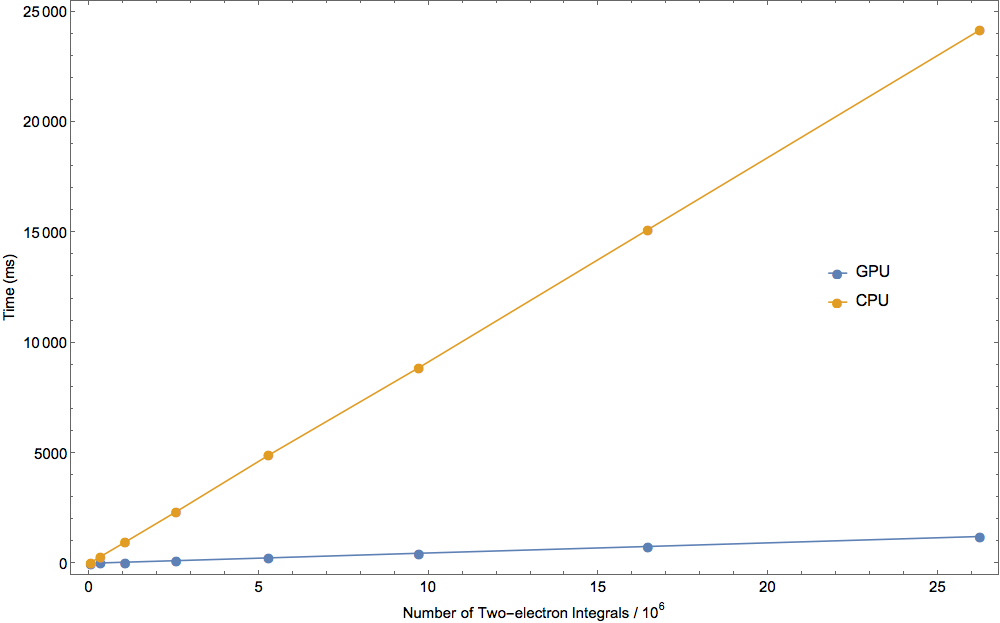
\includegraphics[width=1\textwidth]{Figures/eint2prof.png}
\caption[Profiling of two-electron integral calculations]
{Profiling of two-electron Integral calculations. The results of profiling the calculation of growing amounts of two-electron integrals. The blue line shows the time needed for GPU calculations and the yellow line shows time needed for CPU calculations. The time for the GPU calculations is the combined time of the \kernel{eint2} and \kernel{binary\_search} kernels.}
\label{fig:2eintprof}
\end{figure}

As can be seen, the GPU calculations of the two-electron integrals outperform the CPU calculations with an average speedup factor of over 19. For calculations with fewer number of integrals to compute the speedup is not as dramatic. This is most likely due to the overhead involved in just starting a GPU kernel. Table \ref{tab:2eintprof} shows two different speedups: one for just calculation of the integrals, and one that shows the speedup if the time needed for \kernel{binary\_search} is included. The time needed to evaluate indices does not have much of an impact on the total performance on the total calculation time which proves this was a good way to generate the $lmpqrs$ indices. Additionally, because cudaDFRATOM is a basis set optimizer, \kernel{binary\_search} will need to be called only once, whereas \kernel{eint2} may need to be called many hundreds of times. Therefore, for an optimization calculation (which the original program is incapable of doing) the total speedup will limit to the just the integral calculations.

\subsection{P and Q Matrix Formation Performance}
As explained in section \ref{sec:PQmeth}, there were two different attempts to speedup the formation of \textbf{P} and \textbf{Q}. The results of these attempts are shown in Tables \ref{tab:PQprofalg1} and \ref{tab:PQprofalg2} and also in Figure \ref{fig:formpqprof}.

\begin{table}[h!]
\begin{center}
\caption[\kernel{MTSE} kernel profiling results.]{\kernel{MTSE} kernel profiling results. Times are in ms. Times are given as the average time needed for a singel iteration from one calculation.}
\label{tab:PQprofalg1}
\begin{tabular}{rrrr}
\toprule
	Two-Electron Integrals	&	Time per Iteration CPU	&	Time per Iteration GPU	&	Speedup	\\
\midrule
	74305	&	1.90		&	6.06		&	0.31		\\
	353220	&	5.78		&	14.25	&	0.40		\\
	1081185	&	18.42	&	27.81	&	0.66		\\
	2588950	&	39.47	&	53.95	&	0.73		\\
	5299140	&	81.05	&	96.13	&	0.84		\\
	9726255	&	152.50	&	173.64	&	0.87		\\
	16476670	&	266.53	&	291.79	&	0.91		\\
	26248635	&	426.25	&	459.38	&	0.92		\\
\bottomrule
\end{tabular}
\end{center}
\end{table}

\begin{table}[h!]
\begin{center}
\caption[\kernel{STSE} kernel profiling results.]{\kernel{STSE} kernel profiling results. Times are in ms. Times are given as the average time needed for a singel iteration from one calculation.}
\label{tab:PQprofalg2}
\begin{tabular}{rrrr}
\toprule
	Two-Electron Integrals	&	Time per Iteration CPU		&	Time per Iteration GPU	&	Speedup	\\
\midrule
	74305	&	1.90		&	2.94		&	0.64	\\
	353220	&	5.78		&	7.56		&	0.76	\\
	1081185	&	18.42	&	15.34	&	1.20	\\
	2588950	&	39.47	&	26.32	&	1.49	\\
	5299140	&	81.05	&	39.45	&	2.05	\\
	9726255	&	152.50	&	88.78	&	1.71	\\
	16476670	&	266.53	&	135.64	&	1.96	\\
	26248635	&	426.25	&	193.99	&	2.19	\\
\bottomrule
\end{tabular}
\end{center}
\end{table}

\begin{figure}[h!]
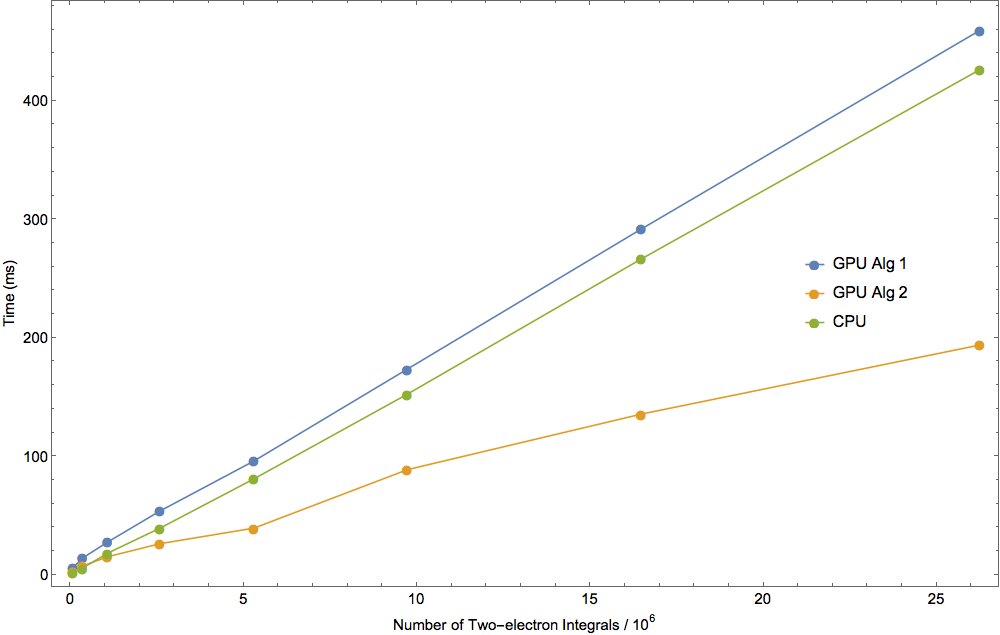
\includegraphics[width=1\textwidth]{Figures/formpqprof.png}
\caption[Profiling of the \kernel{formpq} kernels.]
{Profiling of the \kernel{formpq} kernels. The results of profiling the formation of the \textbf{P} and \textbf{Q} matrices. The blue line shows the time needed for GPU calculations using the \kernel{MTSE} algorithm, the yellow line shows time needed for GPU calculations using \kernel{STSE}, and the green line shows the time needed for the CPU. Because the GPU calculations converge in fewer SCF iterations than the CPU calculations, only the average time for one iteration is shown.}
\label{fig:formpqprof}
\end{figure}

As can be seen, the attempt at \kernel{MTSE} was a complete failure and it isn't even faster than the CPU calculations. \kernel{STSE} was much better, but only just. It achieves little more than a two-fold speedup at best. 

There are several reasons this could be the case. The first due to the poor global memory access that reading $x$ has. $x$ is stored as a vector. This helps greatly with memory cost and integral calculation, but makes it difficult to retrieve it as if it were a matrix.There is the cost of calculating where the necessary integral is, and then the cost of the very uncoalesced reads. Calculating the integrals as a vector, and then copying them into a matrix afterwards could help with this, but the large amount of integrals needed for large calculations makes this impractical on current hardware. How much of an effect inefficient access of global memory has on a calculation does have a limit however which is most likely why the speedup sees an improvement as the calculations get larger. A second reason that the speedup is limited is caused by the occupancy that the kernels can achieve on the GPU. A block size of 512 means that there is a maximum number of 3 blocks running per SM at a time. But these kernels are both limited by the register usage to just running one block per SM at a time. This is also most likely why \kernel{MTSE} performs so poorly compared \kernel{STSE}. \kernel{MTSE} was designed to spread out the amount of work to as many threads as possible. This results in a lot of blocks to be run. But because the amount of blocks that can run at a time is so limited there is no chance to see an improvement. But in the case of \kernel{STSE}, there are a fewer number of blocks needing be be run, although each one needs to run for longer than those of \kernel{MTSE}. Overall \kernel{MTSE} comes out on top.

\begin{figure}
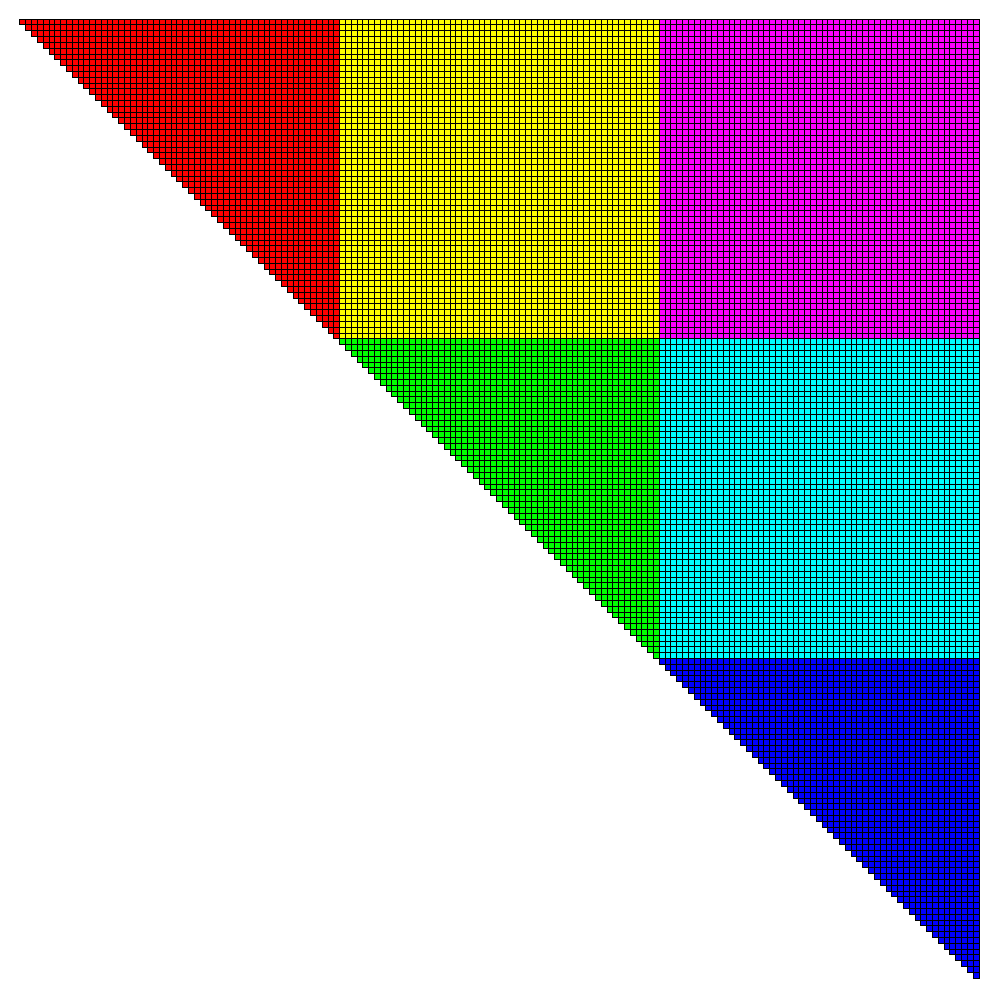
\includegraphics[width=1\textwidth]{Figures/eint2_mat_lots.png}
\caption[Integrals needed for the first element of \textbf{P}: matrix representation]
{Integrals needed for the first element of \textbf{P}: The top triangle of the symmetric two-electron integral matrix in a matrix representation. The required integrals have been highlighted with a green border. The basis set used had $nsym=3$ with $nbs(i) = (10, 10, 10)$. For clarity, the boxes have been coloured based on the spinor symmetries that they contain.}
\label{fig:eint2matlots}
\end{figure}

\begin{figure}
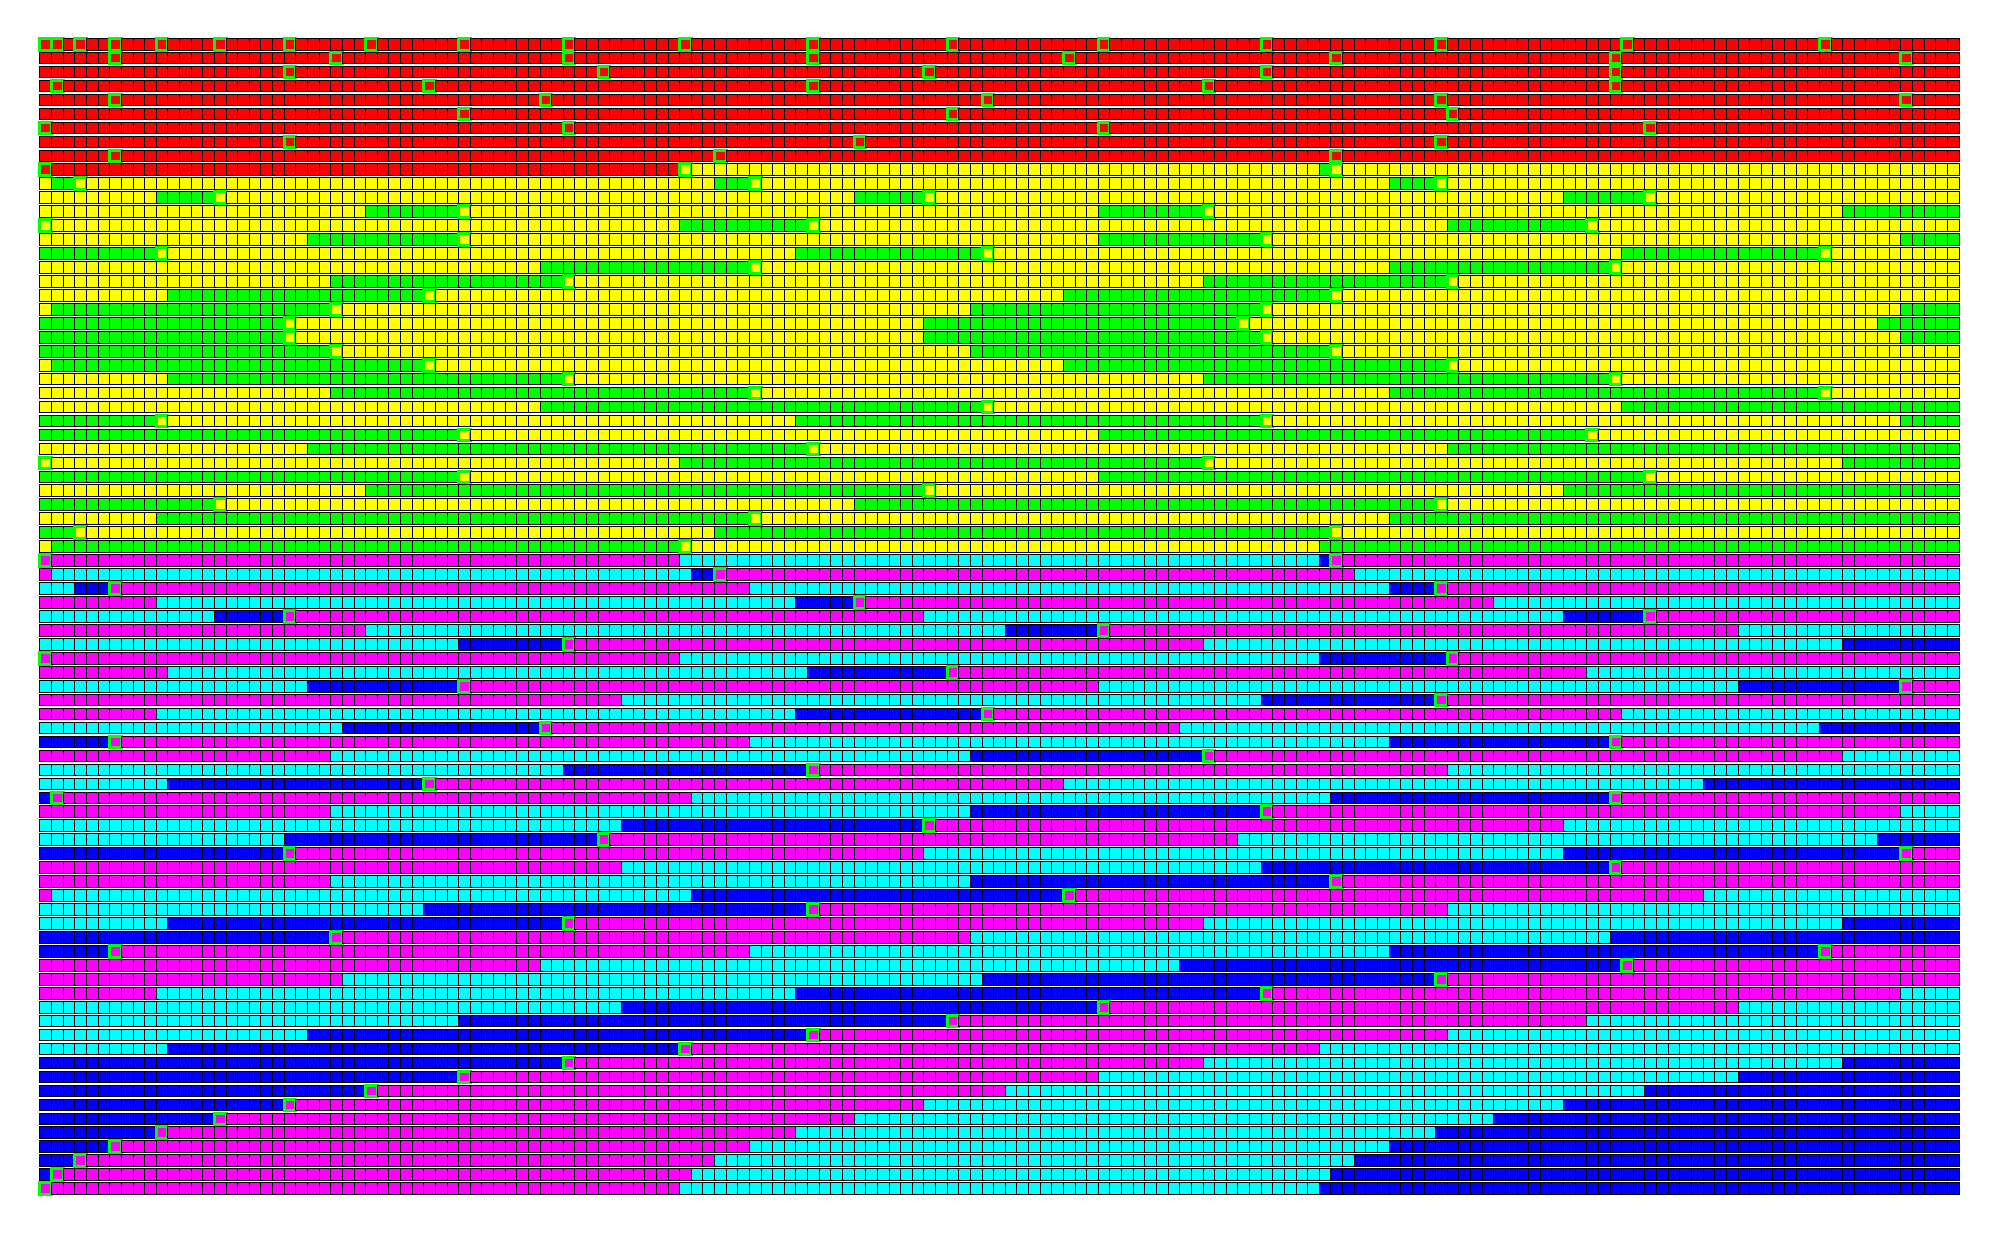
\includegraphics[width=1\textwidth]{Figures/eint2_vec_lots.png}
\caption[Integrals needed for the first element of \textbf{P}: vector representation]
{Integrals needed for the first element of \textbf{P}: The top triangle of the symmetric two-electron integral matrix in a vector representation. The required integrals have been highlighted with a green border.  The spreading out of the elements means that reads to them can not be done effectively. The basis set used had $nsym=3$ with $nbs(i) = (10, 10, 10)$. For clarity, the boxes have been coloured in the same way as Figure \ref{fig:eint2matlots}.}
\label{fig:eint2veclots}
\end{figure}


At present, the limitations of these algorithms are caused by the hardware they run on, not the efficiency of the algorithms themselves. If we imagine removing these limitations, we could consider which one will be better. I propose that \kernel{MTSE} will eventually surpass \kernel{STSE} for very large systems for the following reasons: the time it takes for a single block of \kernel{MTSE} to run is mostly governed by how well it can read the $x$ vector. The effect of spreading out the elements has on memory bandwidth has a limit, once the elements are spread out enough, spreading them out further has no impact. Therefore there is a maximum amount of time it takes for a single block to run. The time for a single block of \kernel{STSE} on the other hand is controlled by both the efficiency of reading global memory \textit{and} the amount of two-electron integrals it must read though. So there is no limit to how long a block can take. Therefore, I predict that \kernel{MTSE} should be faster as the number of integrals becomes very large.

\subsection{Total Speedup}
There was some difficulty in determining the total speedup of a calculation. The reason why can be seen in Tables \ref{tab:totalprofalg1} and \ref{tab:totalprofalg2}.

\begin{table}[h!]
\begin{center}
\caption[Total speedup of alg1]{Total speedup of cudaDFRATOM using \textbf{MTSE}. The results for a total calculation are shown. All times are in s. Times are given as the average time needed for five calculations.}
\label{tab:totalprofalg1}
\begin{tabular}{rrrrrr}
\toprule
	\multirow{2}{3cm}{Two-Electron Integrals}	&	\multirow{2}{3cm}{SCF Iterations CPU}	&	\multirow{2}{2cm}{Total CPU Time}		&	\multirow{2}{3cm}{SCF Iteractions GPU}		&	\multirow{2}{2cm}{Total GPU Time}		&	\multirow{2}{*}{Speedup}	\\
	\\
\midrule
	74305	&	21	&	0.12		&	21	&	0.84	&	0.14	\\
	353220	&	19	&	0.49		&	19	&	1.19	&	0.41	\\
	1081185	&	19	&	1.44		&	19	&	1.75	&	0.82	\\
	2588950	&	19	&	3.38		&	19	&	2.58	&	1.30	\\
	5299140	&	19	&	6.78		&	19	&	3.80	&	1.78	\\
	9726255	&	24	&	13.29	&	19	&	5.77	&	2.30	\\
	16476670	&	26	&	23.23	&	19	&	8.60	&	2.69	\\
	26248635	&	24	&	35.63	&	19	&	12.5	&	2.82	\\
\bottomrule
\end{tabular}
\end{center}
\end{table}

\begin{table}[h!]
\begin{center}
\caption[Total speedup of alg2]{Total speedup of cudaDFRATOM using \textbf{STSE}. The results for a total calculation are shown. All times are in s.}
\label{tab:totalprofalg2}
\begin{tabular}{rrrrrr}
\toprule
	\multirow{2}{3cm}{Two-Electron Integrals}	&	\multirow{2}{3cm}{SCF Iterations CPU}	&	\multirow{2}{2cm}{Total CPU Time}		&	\multirow{2}{3cm}{SCF Iteractions GPU}		&	\multirow{2}{2cm}{Total GPU Time}		&	\multirow{2}{*}{Speedup}	\\
	\\
\midrule
	74305	&	21	&	0.12		&	21	&	0.78	&	0.15	\\
	353220	&	19	&	0.49		&	19	&	1.07	&	0.46	\\
	1081185	&	19	&	1.44		&	19	&	1.51	&	0.95	\\
	2588950	&	19	&	3.38		&	19	&	2.08	&	1.62	\\
	5299140	&	19	&	6.78		&	19	&	2.72	&	2.49	\\
	9726255	&	24	&	13.29	&	19	&	4.14	&	3.20	\\
	16476670	&	26	&	23.23	&	19	&	5.57	&	4.16	\\
	26248635	&	24	&	35.63	&	19	&	7.47	&	4.76	\\
\bottomrule
\end{tabular}
\end{center}
\end{table}

\begin{figure}[h!]
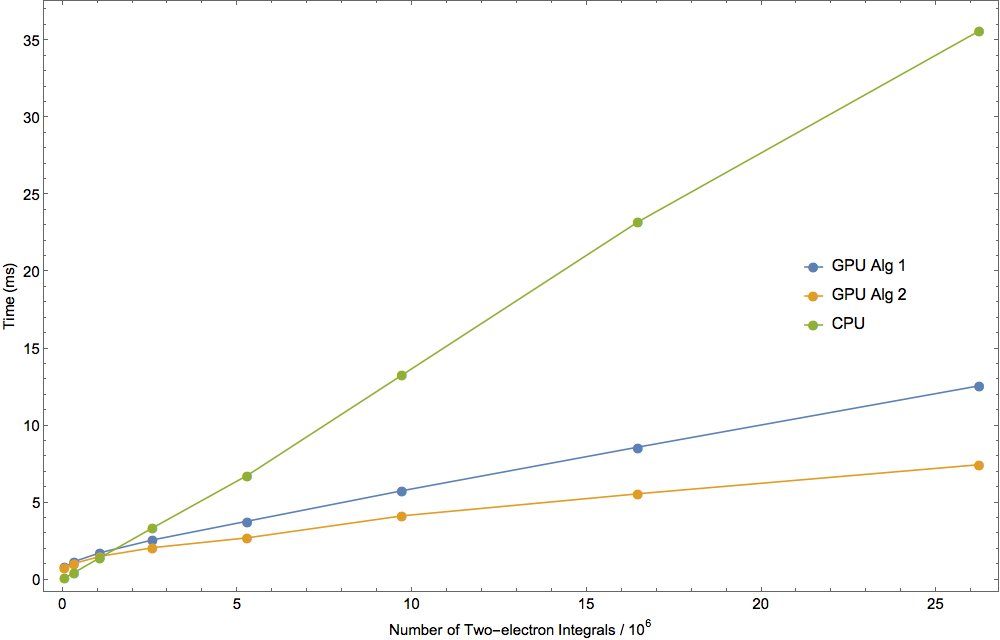
\includegraphics[width=1\textwidth]{Figures/totaltimeprof.png}
\caption[Total time need to complete a calculation.]
{Total time need to complete a calculation.}
\label{fig:totaltimeprof}
\end{figure}

As can be seen, the number of SCF iterations differs when comparing the GPU calculations to the CPU even though the convergence criteria was exactly the same. This is somewhat puzzling but I offer the following explanation. The differences do not occur in the two-electron integral calculations. We confirmed this by comparing the sum of the absolute values of the integrals from both the GPU and non-GPU programs and found that they were the same. The problem instead occurs as a result of changing the SCF routines. First, when writing the SCF routines, it became apparent that rewriting the linear algebra into CUDA would be rather pointless when I could just use the cuSOLVER and cuBLAS libraries and achieve the same result. As such, the SCF is completed using entirely different algorithms and unfortunately, these GPU libraries do not produce exactly the same eigenvalues as the original program. Second, it is important to realize that a real number can only be \textit{approximated} using double precision variables. This introduces numerical instability. For instance, assume that we have a computer that could only hold the first four digits of a number (leading zeros don't count). Then we take the number 1.000 and we want to add 0.0001000 to it 10000 times. The result of the first addition should be 1.0001, but because our computer can only hold four digits, the number is truncated to 1.000. The final result of this computation would not be 2.000 as expected but 1.000. During an SCF calculation, there are millions of numbers being multiplied together and added up, many of which may be close to, but not quite 0. This allows for lots of error to creep into a calculation just because of the limitations of the hardware. 

The fact that two different algorithms are being used on the GPU and CPU, and that they might not be handling numerical stability in the same way is what is most likely causing this to occur. It should also be pointed out that the final energy was not exactly the same from GPU to CPU either. Typically, the last 4 of 16 significant digits would be different. Because the rest are the same however, we still have ``chemical accuracy" (the general consensus of chemical accuracy is $0.001$ Hartree, which cudaDFRATOM falls well within) and I argue that cudaDFRATOMs results are therefore valid.


\section{Input Description}\label{inp_des}
cudaDFRATOM can be executed on Unix-like systems in the following way
\begin{lstlisting}[language=bash]
	$ path_to_executable input_file > output_file
\end{lstlisting}

The input file must end in ``.inp" or an error will be given. Redirection of stdout to an output file is optional, but is recommended to save the results of a calculation. The input file is read using the namelist functionality of Fortran. A description of what must appear on each line of the input file is given below. Sample input files are also given in Appendix \ref{app:cudaDFRATOM_inp}.

\begin{enumerate}
	\item A title of no more than 200 characters.
	\item	\$contrl	\\
				\\
		\begin{tabular}{\vartables}
			jobtype	&		&			&	The type of calculation to be performed.							\\
					&	=	& 	'energy'	& 	Will do a single point energy calculation.							\\
					&	=	&	'bsopt'	& 	Will optimize the basis set. Can only be used if bastype equals 'wtbs'.	\\
			c		&		&			&	The speed of light. If not given, the default is set to 137.03599976 au.	\\
		\end{tabular}
	\item \$nuc	\\
				\\
		\begin{tabular}{\vartables}
			znuc		&		&		&	The charge of the nucleus.									\\
			nucmdl	&		& 		&	The nuclear model to use.										\\
					&	=	&	1	&	Point nucleus (default).										\\
					&	=	&	2	&	Finite sphere (not yet supported). 								\\
					&	=	&	3	&	Gaussian.													\\
			rnuc		&		&		&	The radius of the finite sphere nucleus.							\\	
			alpha	&		&		&	The exponent for the gaussian nucleus. Defaults are given in litdata.f90.	\\				
		\end{tabular}
	\item \$bas	\\
				\\
			\begin{tabular}{\vartables}
			nsym	&		&			&	The number of symmetries to be used.							\\
			bastype	&		& 			&	The type of basis set given.									\\
					&	=	&	'wtbs'	&	Use a WTBS basis set.										\\
					&	=	&	'rdin'		&	Read in the basis set from the input file.							\\
			ngroup	&		&			&	The number of different groups to use in the WTBS scheme (default 1).	\\			
		\end{tabular}
		\\			
		The next line will depend on the value of bastype. If bastype equals `rdin' then the following lines must be the number of functions for the S+ symmetry, followed by the exponents to use, each on a new line. The pattern repeats for each new symmetry. See the sample input files for further clarification. Otherwise, if bastype equals `WTBS' the \$wtbs group is read next.
		
	\item \$wtbs has to be given if bastype='wtbs'.	\\
										\\
		\begin{tabular}{\vartables}
			wtbspara	&		&	&	The $\alpha$, $\beta$, $\delta$, and $\gamma$ WTBS parameters.
									If there is more than one group, the order would be  $\alpha_{1}$, $\beta_{1}$, 
									$\delta_{1}$, $\gamma_{1}$,  $\alpha_{2}$, $\beta_{2}$, $\delta_{2}$, $\gamma_{2}$ 
									and so on.																	\\
			nbs		&		& 	&	The number of functions used in each symmetry.									\\
			start		&		&	&	Where in the $\zeta$ pool each symmetry starts taking exponents from (default=1,1,1,1,1,1,1).	\\
			groups	&		&	&	What group each symmetry belongs to (default=1,1,1,1,1,1,1).							\\
		\end{tabular}
		\\
		The next line depends on what the jobtype was set to. If jobtype equals 'energy' \$newuoa is skipped and \$econfig will be read next. If jobtype equals `bsopt', then the \$newuoa group will be needed.
		
		\item \$newuoa has to be given if jobtype='bsopt'. Refer to the newuoa documentation \cite{Powell2006} for detailed information if needed.	\\
												\\
		\begin{tabular}{\vartables}
			rhobeg	&		&		&	The initial value of the trust region used by newuoa (default=0.1).									\\
			rhoend	&		& 		&	The final value of the trust region used by newuoa. Must be smaller
										than rhobeg (default=$1.0\times{}10^{-4}$).			\\
			iprint		&		&		&	The print level for newuoa.													\\
					&	=	&	0	&	No printing from newuoa (default).												\\
					&	=	&	1	&	Print only when newuoa has finished.											\\
					&	=	&	2	&	Print only when the trust region has decreased by an order of magnitude.					\\
					&	=	&	3	&	Print every iteration of newuoa.													\\
			maxfun	&		&		&	The maximum number of calls to calfun newuoa will make before terminating (default=500).	\\
		\end{tabular}
		\\
		\item \$econfig
		\\
		\begin{tabular}{\vartables}
			nclose	&		&		&	The number of closed spinors for each symmetry.										\\
			nopen	&		& 		&	The number of open spinors for each symmetry. There is a limit to one open orbital per symmetry.	\\
			freeel	&		&		&	The number of electrons available in the open spinors.									\\
			autogen	&		&		&	Automatically generates all possible combinations of spinor occupancies (default=.false.).			\\
			nconf	&		&		&	The number of configurations to be read in (needed if autogen is false).						\\
		\end{tabular}
		\\
		If autogen is false, then the next nconf lines will be the spinor occupancies. They will be given as real numbers with one configuration per line.
		\\
		\\
		\item \$scf
		\\
		\begin{tabular}{\vartables}
			maxitr	&		&		&	The maximum number of SCF iterations (default=50).									\\
			ixtrp		&		& 		&	The method of extrapolation.														\\
					&	=	&	0	&	No extrapolation (default).															\\
					&	=	&	1	&	Extrapolate the Fock matrix.														\\
			dfctr		&		&		&	Damping factor for Fock maxtrix (default=0.3).											\\
			thdll		&		&		&	Convergence limit for the large-large components of the density matrix (default=$1.0\times10^{-5}$)	\\
			thdsl		&		&		&	Convergence limit for the small-large components of the density matrix (default=$1.0\times10^{-7}$)	\\
			thdss	&		&		&	Convergence limit for the small-small components of the density matrix (default=$1.0\times10^{-9}$)	\\
		\end{tabular}
		\\
\end{enumerate}
